%
% main.tex -- Paper zum Thema <zeta>
%
% (c) 2020 Hochschule Rapperswil
%
\chapter{Riemannsche Zetafunktion\label{chapter:zeta}}
\lhead{Riemannsche Zetafunktion}
\begin{refsection}
\chapterauthor{Raphael Unterer}




\section{Einleitung}
\rhead{Einleitung}
Heutzutage ist die Navigation ein Teil des Lebens. 
\index{Navigation}%
Man sendet dem Kollegen seinen eigenen Standort, um sich das ewige Erklären zu sparen oder gibt die Adresse des Ziels ein, damit man seinen Aufenthaltsort zum Beispiel auf einer riesigen Wiese am See findet. 
Dies wird durch Technologien wie Funknavigation, welches ein auf Laufzeitmessung beruhendes Hyperbelverfahren mit Langwellen ist, oder die verbreitete Satellitennavigation, welche vier Satelliten für eine Messung zur Standortbestimmung nutzt.
\index{Funknavigation}%
\index{GPS}%
Vor all diesen technologischen Fortschritten gab es lediglich die Astronavigation, welche heute noch auf Schiffen verwendet wird im Falle eines Stromausfalls. 
Aber wie funktioniert die Navigation mit den Sternen? Welche Hilfsmittel benötigt man, welche Rolle spielt die Mathematik und weshalb kann die Erde nicht flach sein? 
In diesem Kapitel werden genau diese Fragen mithilfe des nautischen Dreiecks, der sphärischen Trigonometrie und einigen Hilfsmitteln und Messgeräten beantwortet.
\index{sphärische Trigonometrie}%

\section{Eulerprodukt} \label{zeta:section:eulerprodukt}
\kopfrechts{Eulerprodukt}

Das Euler-Produkt stellt die gesuchte Verbindung der Zeta-Funktion und der Primzahlen her.
\index{Euler-Produkt}%
Wie der Name bereits sagt, wurde das Eulerprodukt bereits 1727 von Euler entdeckt.
Um daraus die Riemannsche Vermutung herzuleiten, wäre aber noch einiges mehr nötig.

\begin{satz}
    Für alle Zahlen $s$ mit $\Re(s) > 1$ ist die Zeta-Funktion identisch mit dem unendlichen Eulerprodukt
    \begin{equation}\label{zeta:eq:eulerprodukt}
        \zeta(s)
        =
        \sum_{n=1}^\infty
        \frac{1}{n^s}
        =
        \prod_{p \in P}
        \frac{1}{1-p^{-s}}
    \end{equation}
    wobei $P$ die Menge aller Primzahlen darstellt.
\index{Menge der Primzahlen}%
\end{satz}

\begin{proof}[Beweis]
    Der Beweis startet mit dem Eulerprodukt und stellt dieses so um, dass die Zeta-Funktion erscheint.
    Als erstes ersetzen wir die Faktoren durch geometrische Reihen
    \begin{equation}
        \prod_{p\in P}
        \frac{1}{1-p^{-s}}
        =
        \prod_{p \in P}
        \sum_{k_p=0}^{\infty}
        \biggl(
        \frac{1}{p^s}
        \biggr)^{k_p}
        =
        \prod_{p \in P}
        \sum_{k_p=0}^{\infty}
        \frac{1}{p^{s k_p}},
    \end{equation}
    dabei iteriert der Index $i$ über alle Primzahlen $p_i$.
    Durch Ausschreiben der Multiplikation und Ausklammern der Summen erhalten wir
    \begin{align}
        \prod_{p \in P}
        \sum_{k_p=0}^{\infty}
        \frac{1}{p^{s k_p}}
        &=
        \sum_{k_2=0}^{\infty}
        \frac{1}{2^{s k_2}}
        \sum_{k_3=0}^{\infty}
        \frac{1}{3^{s k_3}}
        \sum_{k_5=0}^{\infty}
        \frac{1}{5^{s k_5}}
        \sum_{k_7=0}^{\infty}
        \frac{1}{7^{s k_7}}
        \ldots
        \nonumber \\
        &=
        \sum_{k_2=0}^{\infty}
        \sum_{k_3=0}^{\infty}
        \sum_{k_5=0}^{\infty}
        \ldots
        \biggl(
        \frac{1}{2^{k_2}}
        \frac{1}{3^{k_3}}
        \frac{1}{5^{k_5}}
        \ldots
        \biggr)^s.
        \label{zeta:equation:eulerprodukt2}
    \end{align}
    Der Fundamentalsatz der Arithmetik (Primfaktorzerlegung) besagt, dass jede beliebige Zahl $n \in \mathbb{N}$ durch eine eindeutige Primfaktorzerlegung
    \begin{equation}
        n = \prod_p p^{k_p} \qquad \forall \; n \in \mathbb{N}
    \end{equation}
beschrieben werden kann.
    Jeder Summand der Summen in \eqref{zeta:equation:eulerprodukt2} ist somit der Kehrwert genau einer natürlichen Zahl $n \in \mathbb{N}$.
    Da die Summen alle möglichen Kombinationen von Exponenten und Primzahlen in \eqref{zeta:equation:eulerprodukt2} enthält, haben wir
    \begin{equation}
        \sum_{k_2=0}^{\infty}
        \sum_{k_3=0}^{\infty}
        \sum_{k_5=0}^{\infty}
        \ldots
        \biggl(
        \frac{1}{2^{k_2}}
        \frac{1}{3^{k_3}}
        \frac{1}{5^{k_5}}
        \ldots
        \biggr)^s
        =
        \sum_{n=1}^\infty
        \frac{1}{n^s}
        =
        \zeta(s),
    \end{equation}
    wodurch das Eulerprodukt bewiesen ist.
\end{proof}


\section{Zusammenhang mit der Gammafunktion} \label{zeta:section:zusammenhang_mit_gammafunktion}
\rhead{Zusammenhang mit der Gammafunktion}

In diesem Abschnitt wird gezeigt, wie sich die Zetafunktion durch die Gammafunktion $\Gamma(s)$ ausdrücken lässt.
Dieser Zusammenhang der Art $\zeta(s) = f(\Gamma(s))$ ist nicht nur interessant, er wird später auch für die Herleitung der analytischen Fortsetzung gebraucht.

Wir erinnern uns an die Definition der Gammafunktion in \eqref{buch:rekursion:gamma:integralbeweis}
\begin{equation*}
    \Gamma(s)
    =
    \int_0^{\infty} t^{s-1} e^{-t} \,dt,
\end{equation*}
wobei die Notation an die Zetafunktion angepasst ist.
Durch die Substitution von $t$ mit $t = nu$ und $dt = n\,du$ wird daraus
\begin{align*}
    \Gamma(s)
    &=
    \int_0^{\infty} n^{s-1}u^{s-1} e^{-nu} n \,du \\
    &=
    \int_0^{\infty} n^s u^{s-1} e^{-nu} \,du.
\end{align*}
Durch Division mit durch $n^s$ ergibt sich die Quotienten
\begin{equation*}
    \frac{\Gamma(s)}{n^s}
    =
    \int_0^{\infty} u^{s-1} e^{-nu} \,du,
\end{equation*}
welche sich zur Zetafunktion summieren
\begin{equation}
    \sum_{n=1}^{\infty} \frac{\Gamma(s)}{n^s}
    =
    \Gamma(s) \zeta(s)
    =
    \int_0^{\infty} u^{s-1}
    \sum_{n=1}^{\infty}e^{-nu}
    \,du.
    \label{zeta:equation:zeta_gamma1}
\end{equation}
Die Summe über $e^{-nu}$ können wir als geometrische Reihe schreiben und erhalten
\begin{align}
    \sum_{n=1}^{\infty}\left(e^{-u}\right)^n
    &=
    \sum_{n=0}^{\infty}\left(e^{-u}\right)^n
    -
    1
    \\
    &=
    \frac{1}{1 - e^{-u}} - 1
    \\
    &=
    \frac{1}{e^u - 1}.
\end{align}
Wenn wir dieses Resultat einsetzen in \eqref{zeta:equation:zeta_gamma1} und durch $\Gamma(s)$ teilen, erhalten wir den gewünschten Zusammenhang
\begin{equation}\label{zeta:equation:zeta_gamma_final}
    \zeta(s)
    =
    \frac{1}{\Gamma(s)}
    \int_0^{\infty}
    \frac{u^{s-1}}{e^u -1}
    du \qed
\end{equation}

\section{Analytische Fortsetzung} \label{zeta:section:analytische_fortsetzung}
\rhead{Analytische Fortsetzung}

%TODO missing Text

\subsection{Fortsetzung auf $\Re(s) > 0$} \label{zeta:subsection:auf_bereich_ge_0}
Zuerst definieren die Dirichletsche Etafunktion als
\begin{equation}\label{zeta:equation:eta}
    \eta(s)
    =
    \sum_{n=1}^{\infty}
    \frac{(-1)^{n-1}}{n^s},
\end{equation}
wobei die Reihe bis auf die alternierenden Vorzeichen die selbe wie in der Zetafunktion ist.
Diese Etafunktion konvergiert gemäss dem Leibnitz-Kriterium im Bereich $\Re(s) > 0$, da dann die einzelnen Glieder monoton fallend sind.

Wenn wir es nun schaffen, die sehr ähnliche Zetafunktion mit der Etafunktion auszudrücken, dann haben die gesuchte Fortsetzung.
Die folgenden Schritte zeigen, wie man dazu kommt:
\begin{align}
    \zeta(s)
    &=
    \sum_{n=1}^{\infty}
    \frac{1}{n^s} \label{zeta:align1}
    \\
    \frac{1}{2^{s-1}}
    \zeta(s)
    &=
    \sum_{n=1}^{\infty}
    \frac{2}{(2n)^s} \label{zeta:align2}
    \\
    \left(1 - \frac{1}{2^{s-1}} \right)
    \zeta(s)
    &=
    \frac{1}{1^s}
    \underbrace{-\frac{2}{2^s} + \frac{1}{2^s}}_{-\frac{1}{2^s}}
    + \frac{1}{3^s}
    \underbrace{-\frac{2}{4^s} + \frac{1}{4^s}}_{-\frac{1}{4^s}}
    \ldots
    && \text{\eqref{zeta:align1}} - \text{\eqref{zeta:align2}}
    \\
    &= \eta(s)
    \\
    \zeta(s)
    &=
    \left(1 - \frac{1}{2^{s-1}} \right)^{-1} \eta(s).
\end{align}

\subsection{Fortsetzung auf ganz $\mathbb{C}$} \label{zeta:subsection:auf_ganz}
Für die Fortsetzung auf den Rest von $\mathbb{C}$, verwenden wir den Zusammenhang von Gamma- und Zetafunktion aus \ref{zeta:section:zusammenhang_mit_gammafunktion}.
Wir beginnen damit, die Gammafunktion für den halben Funktionswert zu berechnen als
\begin{equation}
    \Gamma \left( \frac{s}{2} \right)
    =
    \int_0^{\infty} t^{\frac{s}{2}-1} e^{-t} dt.
\end{equation}
Nun substituieren wir $t$ mit $t = \pi n^2 x$ und $dt=\pi n^2 dx$ und erhalten
\begin{align}
    \Gamma \left( \frac{s}{2} \right)
    &=
    \int_0^{\infty}
    (\pi n^2)^{\frac{s}{2}}
    x^{\frac{s}{2}-1}
    e^{-\pi n^2 x}
    dx
    && \text{Division durch } (\pi n^2)^{\frac{s}{2}}
    \\
    \frac{\Gamma \left( \frac{s}{2} \right)}{\pi^{\frac{s}{2}} n^s}
    &=
    \int_0^{\infty}
    x^{\frac{s}{2}-1}
    e^{-\pi n^2 x}
    dx
    && \text{Zeta durch Summenbildung } \sum_{n=1}^{\infty}
    \\
    \frac{\Gamma \left( \frac{s}{2} \right)}{\pi^{\frac{s}{2}}}
    \zeta(s)
    &=
    \int_0^{\infty}
    x^{\frac{s}{2}-1}
    \sum_{n=1}^{\infty}
    e^{-\pi n^2 x}
    dx. \label{zeta:equation:integral1}
\end{align}
Die Summe kürzen wir ab als $\psi(x) = \sum_{n=1}^{\infty} e^{-\pi n^2 x}$.
%TODO Wieso folgendes -> aus Fourier Signal
Es gilt
\begin{equation}\label{zeta:equation:psi}
    \psi(x)
    =
    - \frac{1}{2}
    + \frac{\psi\left(\frac{1}{x} \right)}{\sqrt{x}}
    + \frac{1}{2 \sqrt{x}}.
\end{equation}

Zunächst teilen wir nun das Integral aus \eqref{zeta:equation:integral1} auf als
\begin{equation}\label{zeta:equation:integral2}
    \int_0^{\infty}
    x^{\frac{s}{2}-1}
    \psi(x)
    dx
    =
    \int_0^{1}
    x^{\frac{s}{2}-1}
    \psi(x)
    dx
    +
    \int_1^{\infty}
    x^{\frac{s}{2}-1}
    \psi(x)
    dx,
\end{equation}
wobei wir uns nun auf den ersten Teil konzentrieren werden.
Dabei setzen wir das Wissen aus \eqref{zeta:equation:psi} ein und erhalten
\begin{align}
    \int_0^{1}
    x^{\frac{s}{2}-1}
    \psi(x)
    dx
    &=
    \int_0^{1}
    x^{\frac{s}{2}-1}
    \left(
    - \frac{1}{2}
    + \frac{\psi\left(\frac{1}{x} \right)}{\sqrt{x}}
    + \frac{1}{2 \sqrt{x}}.
    \right)
    dx
    \\
    &=
    \int_0^{1}
    x^{\frac{s}{2}-\frac{3}{2}}
    \psi \left( \frac{1}{x} \right)
    + \frac{1}{2}
    \left(
    x^{\frac{s}{2}-\frac{3}{2}}
    -
    x^{\frac{s}{2}-1}
    \right)
    dx
    \\
    &=
    \int_0^{1}
    x^{\frac{s}{2}-\frac{3}{2}}
    \psi \left( \frac{1}{x} \right)
    dx
    + \frac{1}{2}
    \int_0^1
    x^{\frac{s}{2}-\frac{3}{2}}
    -
    x^{\frac{s}{2}-1}
    dx. \label{zeta:equation:integral3}
\end{align}
Dabei kann das zweite Integral gelöst werden als
\begin{equation}
    \frac{1}{2}
    \int_0^1
    x^{\frac{s}{2}-\frac{3}{2}}
    -
    x^{\frac{s}{2}-1}
    dx
    =
    \frac{1}{s(s-1)}.
\end{equation}
Das erste Integral aus \eqref{zeta:equation:integral3} mit $\psi \left(\frac{1}{x} \right)$ ist nicht lösbar in dieser Form.
Deshalb substituieren wir $x = \frac{1}{u}$ und $dx = -\frac{1}{u^2}du$.
Die untere Integralgrenze wechselt ebenfalls zu $x_0 = 0 \rightarrow u_0 = \infty$.
Dies ergibt
\begin{align}
    \int_{\infty}^{1}
    {\frac{1}{u}}^{\frac{s}{2}-\frac{3}{2}}
    \psi(u)
    \frac{-du}{u^2}
    &=
    \int_{1}^{\infty}
    {\frac{1}{u}}^{\frac{s}{2}-\frac{3}{2}}
    \psi(u)
    \frac{du}{u^2}
    \\
    &=
    \int_{1}^{\infty}
    x^{(-1) \left(\frac{s}{2}+\frac{1}{2}\right)}
    \psi(x)
    dx,
\end{align}
wobei wir durch Multiplikation mit $(-1)$ die Integralgrenzen tauschen dürfen.
Es ist zu beachten das diese Grenzen nun identisch mit den Grenzen des zweiten Integrals von \eqref{zeta:equation:integral2} sind.
Wir setzen beide Lösungen ein in Gleichung \eqref{zeta:equation:integral3} und erhalten
\begin{equation}
    \int_0^{1}
    x^{\frac{s}{2}-1}
    \psi(x)
    dx
    =
    \int_{1}^{\infty}
    x^{(-1) \left(\frac{s}{2}+\frac{1}{2}\right)}
    \psi(x)
    dx,
    +
    \frac{1}{s(s-1)}.
\end{equation}
Dieses Resultat setzen wir wiederum ein in \eqref{zeta:equation:integral2}, um schlussendlich
\begin{align}
    \frac{\Gamma \left( \frac{s}{2} \right)}{\pi^{\frac{s}{2}}}
    \zeta(s)
    &=
    \int_0^{1}
    x^{\frac{s}{2}-1}
    \psi(x)
    dx
    +
    \int_1^{\infty}
    x^{\frac{s}{2}-1}
    \psi(x)
    dx
    \nonumber
    \\
    &=
    \frac{1}{s(s-1)}
    +
    \int_{1}^{\infty}
    x^{(-1) \left(\frac{s}{2}+\frac{1}{2}\right)}
    \psi(x)
    dx,
    +
    \int_1^{\infty}
    x^{\frac{s}{2}-1}
    \psi(x)
    dx
    \\
    &=
    \frac{1}{s(s-1)}
    +
    \int_{1}^{\infty}
    \left(
    x^{-\frac{s}{2}-\frac{1}{2}}
    +
    x^{\frac{s}{2}-1}
    \right)
    \psi(x)
    dx
    \\
    &=
    \frac{-1}{s(1-s)}
    +
    \int_{1}^{\infty}
    \left(
    x^{\frac{1-s}{2}}
    +
    x^{\frac{s}{2}}
    \right)
    \frac{\psi(x)}{x}
    dx,
\end{align}
zu erhalten.
Wenn wir dieses Resultat genau anschauen, erkennen wir dass sich nichts verändert wenn $s$ mit $1-s$ ersetzt wird.
Somit haben wir die analytische Fortsetzung gefunden als
\begin{equation}\label{zeta:equation:functional}
    \frac{\Gamma \left( \frac{s}{2} \right)}{\pi^{\frac{s}{2}}}
    \zeta(s)
    =
    \frac{\Gamma \left( \frac{1-s}{2} \right)}{\pi^{\frac{1-s}{2}}}
    \zeta(1-s).
\end{equation}


\section{Der Wert $\zeta(-1)$} \label{zeta:section:fazit}
\rhead{Der Wert $\zeta(-1)$}
\index{zeta(-1)@$\zeta(-1)$}%

Ganz zu Beginn dieses Papers wurde die Behauptung erwähnt, dass die Summe aller natürlichen Zahlen $-\frac{1}{12}$ sei.
Diese Summe ist nichts anderes als die Zeta-Funktion am Wert $s=-1$.
Da wir die analytische Fortsetzung mit der Funktionalgleichung \eqref{zeta:equation:functional} gefunden haben, können wir den Wert $s=-1$ einsetzen und erhalten
\begin{align*}
    \zeta(s)
    &=
    \frac{\Gamma ( \frac{1-s}{2} )}{\pi^{\frac{1-s}{2}}}
    \zeta(1-s)
    \frac{\pi^{\frac{s}{2}}}{\Gamma ( \frac{s}{2} )}
    \\
    \zeta(-1)
    &=
    \frac{\Gamma(1)}{\pi}
    \zeta(2)
    \frac{\pi^{-\frac{1}{2}}}{\Gamma ( -\frac{1}{2} )}.
\end{align*}
Also fehlen uns drei Werte, $\zeta(2)$, $\Gamma(1)$ und $\Gamma(-\frac{1}{2})$.

Zunächst konzentrieren wir uns auf $\zeta(2)$, welches im konvergenten Bereich der Reihe liegt und auch bekannt ist als das Basler Problem.
\index{Basler Problem}%
Wir lösen das Basler Problem \cite{zeta:online:basel} mithilfe der parsevalschen Gleichung \cite{zeta:online:pars}
\index{parsevalsche Gleichung}%
\begin{align}
    \int_{-\pi}^{\pi} |f(x)|^2 dx
    &=
    2\pi \sum_{n=-\infty}^{\infty} |c_n|^2 \\
    c_n
    &=
    \frac{1}{2\pi}
    \int_{-\pi}^{\pi}f(x)e^{-inx} dx,
\end{align}
welche besagt dass die Summe der quadrierten Fourierkoeffizienten einer Funktion identisch ist mit dem Integral der quadrierten Funktion.
Wenn wir dies für $f(x) = x$ auswerten erhalten wir
\begin{align}
    c_n
    &=
    \begin{cases}
        \frac{(-1)^n}{n} i, & \text{for } n\neq0, \\
        0, & \text{for } n=0
    \end{cases}
    \\
    \int_{-\pi}^{\pi} x^2 dx
    &=
    2\pi \sum_{n=-\infty}^{\infty} |c_n|^2
    =
    4\pi \underbrace{\sum_{n=1}^{\infty} \frac{1}{n^2}}_{\displaystyle{\zeta(2)}}.
\end{align}
Durch einfaches Umstellen erhalten wir somit die Lösung des Basler Problems als
\begin{equation}
    \zeta(2) = \sum_{n=1}^{\infty} \frac{1}{n^2} = \frac{1}{4\pi}
    \int_{-\pi}^{\pi} x^2 dx
    = \frac{\pi^2}{6}.
\end{equation}

Als nächstes berechnen wir $\Gamma(1)$ und $\Gamma(-\frac{1}{2})$ mithilfe der Integraldefinition der Gamma-Funktion (Definition \ref{buch:rekursion:def:gamma}).
Da das Integral für $\Gamma(-\frac{1}{2})$ nicht konvergiert, wird die Reflektionsformel aus \ref{buch:funktionentheorie:subsection:gammareflektion} verwendet, welche das konvergierende Integral von  $\Gamma(\frac{3}{2})$ verwendet.
Es ergeben sich die Werte
\begin{align*}
    \Gamma(1)
    &= 1\\
    \Gamma\biggl(-\frac{1}{2}\biggr)
    &= \frac{\pi}{\sin(-\frac{\pi}{2})
    \Gamma(\frac{3}{2})}
    = -\frac{\sqrt{\pi}}{2}.
\end{align*}

Wenn wir diese Werte in die Funktionalgleichung einsetzen, erhalten wir das gewünschte Ergebnis
\begin{align*}
    \zeta(-1)
    &=
    \frac{\Gamma(1)}{\pi}
    \zeta(2)
    \frac{\pi^{-\frac{1}{2}}}{\Gamma ( -\frac{1}{2} )}
    \\
    &=
    \frac{1}{\pi}
    \frac{\pi^2}{6}
    \frac{\pi^{-\frac{1}{2}}}{
    -\frac{\sqrt{\pi}}{2}}
    \\
    &=
    -\frac{1}{12}.
\end{align*}

Weiter wurde zu Beginn dieses Papers auf die Riemannsche Vermutung hingewiesen, wonach alle nichttrivialen Nullstellen der Zeta-Funktion auf der $\Re(s)=\frac{1}{2}$ Geraden der komplexen Ebene liegen.
Abbildung \ref{zeta:fig:einzweitel} zeigt die Funktionswerte dieser Geraden.
\begin{figure}
    \centering
    %%
% zetaplot.tex -- Abbildung der kritischen Geraden
%
% (c) 2021 Prof Dr Andreas Müller, OST Ostschweizer Fachhochschule
%
\documentclass[tikz]{standalone}
\usepackage{amsmath}
\usepackage{times}
\usepackage{txfonts}
\usepackage{pgfplots}
\usepackage{csvsimple}
\usetikzlibrary{arrows,intersections,math}
\begin{document}
\def\skala{1}
\begin{tikzpicture}[>=latex,thick,scale=\skala]

\def\dx{2}
\def\dy{2}

\draw[->] ({-1.6*\dx},0) -- ({3.4*\dx},0)
	coordinate[label={$\Re\zeta(\frac12+it)$}];
\draw[->] (0,{-2.1*\dx}) -- (0,{2.2*\dx})
	coordinate[label={left:$\Im\zeta(\frac12+it)$}];

\foreach \x in {-1,1,2,3}{
	\node at ({\x*\dx},-0.1) [below] {$\x$};
}
\node at (-0.1,{1*\dy}) [above left] {$i$};
\node at (-0.1,{2*\dy}) [left] {$2i$};
\node at (-0.1,{-1*\dy}) [below left] {$-i$};
\node at (-0.1,{-2*\dy}) [left] {$-2i$};

\foreach \x in {-1,1,2,3}{
	\draw ({\x*\dx},-0.1) -- ({\x*\dx},0.1);
}
\foreach \y in {1,2}{
	\draw (-0.1,{\y*\dy}) -- (0.1,{\y*\dy});
	\draw (-0.1,{-\y*\dy}) -- (0.1,{-\y*\dy});
}

\def\zetapath{
 ({-1.4604*\dx},{0.0000*\dy})
	-- ({-1.4572*\dx},{-0.0783*\dy})
	-- ({-1.4476*\dx},{-0.1559*\dy})
	-- ({-1.4319*\dx},{-0.2320*\dy})
	-- ({-1.4104*\dx},{-0.3058*\dy})
	-- ({-1.3834*\dx},{-0.3769*\dy})
	-- ({-1.3514*\dx},{-0.4446*\dy})
	-- ({-1.3149*\dx},{-0.5085*\dy})
	-- ({-1.2745*\dx},{-0.5682*\dy})
	-- ({-1.2308*\dx},{-0.6235*\dy})
	-- ({-1.1843*\dx},{-0.6742*\dy})
	-- ({-1.1358*\dx},{-0.7202*\dy})
	-- ({-1.0856*\dx},{-0.7617*\dy})
	-- ({-1.0344*\dx},{-0.7985*\dy})
	-- ({-0.9826*\dx},{-0.8309*\dy})
	-- ({-0.9306*\dx},{-0.8591*\dy})
	-- ({-0.8788*\dx},{-0.8833*\dy})
	-- ({-0.8275*\dx},{-0.9037*\dy})
	-- ({-0.7770*\dx},{-0.9205*\dy})
	-- ({-0.7275*\dx},{-0.9341*\dy})
	-- ({-0.6792*\dx},{-0.9446*\dy})
	-- ({-0.6322*\dx},{-0.9525*\dy})
	-- ({-0.5867*\dx},{-0.9578*\dy})
	-- ({-0.5427*\dx},{-0.9609*\dy})
	-- ({-0.5002*\dx},{-0.9620*\dy})
	-- ({-0.4593*\dx},{-0.9613*\dy})
	-- ({-0.4200*\dx},{-0.9589*\dy})
	-- ({-0.3823*\dx},{-0.9552*\dy})
	-- ({-0.3462*\dx},{-0.9502*\dy})
	-- ({-0.3116*\dx},{-0.9441*\dy})
	-- ({-0.2785*\dx},{-0.9371*\dy})
	-- ({-0.2469*\dx},{-0.9292*\dy})
	-- ({-0.2167*\dx},{-0.9206*\dy})
	-- ({-0.1878*\dx},{-0.9114*\dy})
	-- ({-0.1603*\dx},{-0.9017*\dy})
	-- ({-0.1340*\dx},{-0.8916*\dy})
	-- ({-0.1089*\dx},{-0.8811*\dy})
	-- ({-0.0849*\dx},{-0.8703*\dy})
	-- ({-0.0621*\dx},{-0.8593*\dy})
	-- ({-0.0402*\dx},{-0.8481*\dy})
	-- ({-0.0194*\dx},{-0.8367*\dy})
	-- ({0.0004*\dx},{-0.8253*\dy})
	-- ({0.0194*\dx},{-0.8137*\dy})
	-- ({0.0375*\dx},{-0.8022*\dy})
	-- ({0.0549*\dx},{-0.7906*\dy})
	-- ({0.0714*\dx},{-0.7790*\dy})
	-- ({0.0872*\dx},{-0.7675*\dy})
	-- ({0.1024*\dx},{-0.7560*\dy})
	-- ({0.1168*\dx},{-0.7446*\dy})
	-- ({0.1307*\dx},{-0.7333*\dy})
	-- ({0.1439*\dx},{-0.7221*\dy})
	-- ({0.1566*\dx},{-0.7110*\dy})
	-- ({0.1688*\dx},{-0.7000*\dy})
	-- ({0.1805*\dx},{-0.6890*\dy})
	-- ({0.1917*\dx},{-0.6783*\dy})
	-- ({0.2024*\dx},{-0.6676*\dy})
	-- ({0.2127*\dx},{-0.6571*\dy})
	-- ({0.2226*\dx},{-0.6467*\dy})
	-- ({0.2321*\dx},{-0.6364*\dy})
	-- ({0.2412*\dx},{-0.6263*\dy})
	-- ({0.2500*\dx},{-0.6163*\dy})
	-- ({0.2585*\dx},{-0.6064*\dy})
	-- ({0.2666*\dx},{-0.5967*\dy})
	-- ({0.2745*\dx},{-0.5871*\dy})
	-- ({0.2820*\dx},{-0.5777*\dy})
	-- ({0.2893*\dx},{-0.5684*\dy})
	-- ({0.2963*\dx},{-0.5592*\dy})
	-- ({0.3031*\dx},{-0.5501*\dy})
	-- ({0.3096*\dx},{-0.5412*\dy})
	-- ({0.3159*\dx},{-0.5324*\dy})
	-- ({0.3220*\dx},{-0.5237*\dy})
	-- ({0.3279*\dx},{-0.5152*\dy})
	-- ({0.3336*\dx},{-0.5067*\dy})
	-- ({0.3391*\dx},{-0.4984*\dy})
	-- ({0.3445*\dx},{-0.4902*\dy})
	-- ({0.3496*\dx},{-0.4821*\dy})
	-- ({0.3546*\dx},{-0.4742*\dy})
	-- ({0.3595*\dx},{-0.4663*\dy})
	-- ({0.3642*\dx},{-0.4586*\dy})
	-- ({0.3687*\dx},{-0.4510*\dy})
	-- ({0.3732*\dx},{-0.4434*\dy})
	-- ({0.3774*\dx},{-0.4360*\dy})
	-- ({0.3816*\dx},{-0.4287*\dy})
	-- ({0.3857*\dx},{-0.4214*\dy})
	-- ({0.3896*\dx},{-0.4143*\dy})
	-- ({0.3934*\dx},{-0.4073*\dy})
	-- ({0.3972*\dx},{-0.4003*\dy})
	-- ({0.4008*\dx},{-0.3935*\dy})
	-- ({0.4043*\dx},{-0.3867*\dy})
	-- ({0.4078*\dx},{-0.3800*\dy})
	-- ({0.4111*\dx},{-0.3734*\dy})
	-- ({0.4144*\dx},{-0.3669*\dy})
	-- ({0.4176*\dx},{-0.3605*\dy})
	-- ({0.4207*\dx},{-0.3541*\dy})
	-- ({0.4237*\dx},{-0.3478*\dy})
	-- ({0.4267*\dx},{-0.3416*\dy})
	-- ({0.4296*\dx},{-0.3355*\dy})
	-- ({0.4324*\dx},{-0.3294*\dy})
	-- ({0.4352*\dx},{-0.3234*\dy})
	-- ({0.4379*\dx},{-0.3175*\dy})
	-- ({0.4405*\dx},{-0.3116*\dy})
	-- ({0.4431*\dx},{-0.3059*\dy})
	-- ({0.4457*\dx},{-0.3001*\dy})
	-- ({0.4482*\dx},{-0.2945*\dy})
	-- ({0.4506*\dx},{-0.2889*\dy})
	-- ({0.4530*\dx},{-0.2833*\dy})
	-- ({0.4554*\dx},{-0.2778*\dy})
	-- ({0.4577*\dx},{-0.2724*\dy})
	-- ({0.4599*\dx},{-0.2670*\dy})
	-- ({0.4622*\dx},{-0.2617*\dy})
	-- ({0.4643*\dx},{-0.2565*\dy})
	-- ({0.4665*\dx},{-0.2513*\dy})
	-- ({0.4686*\dx},{-0.2461*\dy})
	-- ({0.4707*\dx},{-0.2410*\dy})
	-- ({0.4727*\dx},{-0.2359*\dy})
	-- ({0.4747*\dx},{-0.2309*\dy})
	-- ({0.4767*\dx},{-0.2259*\dy})
	-- ({0.4787*\dx},{-0.2210*\dy})
	-- ({0.4806*\dx},{-0.2161*\dy})
	-- ({0.4825*\dx},{-0.2113*\dy})
	-- ({0.4844*\dx},{-0.2065*\dy})
	-- ({0.4862*\dx},{-0.2018*\dy})
	-- ({0.4880*\dx},{-0.1971*\dy})
	-- ({0.4898*\dx},{-0.1924*\dy})
	-- ({0.4916*\dx},{-0.1878*\dy})
	-- ({0.4934*\dx},{-0.1832*\dy})
	-- ({0.4951*\dx},{-0.1786*\dy})
	-- ({0.4968*\dx},{-0.1741*\dy})
	-- ({0.4985*\dx},{-0.1696*\dy})
	-- ({0.5002*\dx},{-0.1652*\dy})
	-- ({0.5019*\dx},{-0.1608*\dy})
	-- ({0.5035*\dx},{-0.1564*\dy})
	-- ({0.5052*\dx},{-0.1521*\dy})
	-- ({0.5068*\dx},{-0.1478*\dy})
	-- ({0.5084*\dx},{-0.1435*\dy})
	-- ({0.5100*\dx},{-0.1392*\dy})
	-- ({0.5116*\dx},{-0.1350*\dy})
	-- ({0.5132*\dx},{-0.1308*\dy})
	-- ({0.5147*\dx},{-0.1267*\dy})
	-- ({0.5163*\dx},{-0.1226*\dy})
	-- ({0.5178*\dx},{-0.1185*\dy})
	-- ({0.5193*\dx},{-0.1144*\dy})
	-- ({0.5208*\dx},{-0.1103*\dy})
	-- ({0.5224*\dx},{-0.1063*\dy})
	-- ({0.5239*\dx},{-0.1023*\dy})
	-- ({0.5254*\dx},{-0.0984*\dy})
	-- ({0.5268*\dx},{-0.0944*\dy})
	-- ({0.5283*\dx},{-0.0905*\dy})
	-- ({0.5298*\dx},{-0.0866*\dy})
	-- ({0.5313*\dx},{-0.0827*\dy})
	-- ({0.5327*\dx},{-0.0789*\dy})
	-- ({0.5342*\dx},{-0.0751*\dy})
	-- ({0.5357*\dx},{-0.0713*\dy})
	-- ({0.5371*\dx},{-0.0675*\dy})
	-- ({0.5386*\dx},{-0.0637*\dy})
	-- ({0.5400*\dx},{-0.0600*\dy})
	-- ({0.5414*\dx},{-0.0563*\dy})
	-- ({0.5429*\dx},{-0.0526*\dy})
	-- ({0.5443*\dx},{-0.0489*\dy})
	-- ({0.5458*\dx},{-0.0453*\dy})
	-- ({0.5472*\dx},{-0.0416*\dy})
	-- ({0.5486*\dx},{-0.0380*\dy})
	-- ({0.5501*\dx},{-0.0344*\dy})
	-- ({0.5515*\dx},{-0.0308*\dy})
	-- ({0.5529*\dx},{-0.0272*\dy})
	-- ({0.5544*\dx},{-0.0237*\dy})
	-- ({0.5558*\dx},{-0.0202*\dy})
	-- ({0.5572*\dx},{-0.0167*\dy})
	-- ({0.5587*\dx},{-0.0132*\dy})
	-- ({0.5601*\dx},{-0.0097*\dy})
	-- ({0.5615*\dx},{-0.0062*\dy})
	-- ({0.5630*\dx},{-0.0028*\dy})
	-- ({0.5644*\dx},{0.0006*\dy})
	-- ({0.5659*\dx},{0.0041*\dy})
	-- ({0.5673*\dx},{0.0075*\dy})
	-- ({0.5688*\dx},{0.0108*\dy})
	-- ({0.5702*\dx},{0.0142*\dy})
	-- ({0.5717*\dx},{0.0176*\dy})
	-- ({0.5731*\dx},{0.0209*\dy})
	-- ({0.5746*\dx},{0.0242*\dy})
	-- ({0.5761*\dx},{0.0275*\dy})
	-- ({0.5776*\dx},{0.0308*\dy})
	-- ({0.5790*\dx},{0.0341*\dy})
	-- ({0.5805*\dx},{0.0374*\dy})
	-- ({0.5820*\dx},{0.0407*\dy})
	-- ({0.5835*\dx},{0.0439*\dy})
	-- ({0.5850*\dx},{0.0471*\dy})
	-- ({0.5865*\dx},{0.0504*\dy})
	-- ({0.5880*\dx},{0.0536*\dy})
	-- ({0.5896*\dx},{0.0568*\dy})
	-- ({0.5911*\dx},{0.0599*\dy})
	-- ({0.5926*\dx},{0.0631*\dy})
	-- ({0.5942*\dx},{0.0663*\dy})
	-- ({0.5957*\dx},{0.0694*\dy})
	-- ({0.5973*\dx},{0.0725*\dy})
	-- ({0.5988*\dx},{0.0757*\dy})
	-- ({0.6004*\dx},{0.0788*\dy})
	-- ({0.6020*\dx},{0.0819*\dy})
	-- ({0.6036*\dx},{0.0850*\dy})
	-- ({0.6052*\dx},{0.0880*\dy})
	-- ({0.6068*\dx},{0.0911*\dy})
	-- ({0.6084*\dx},{0.0942*\dy})
	-- ({0.6100*\dx},{0.0972*\dy})
	-- ({0.6117*\dx},{0.1002*\dy})
	-- ({0.6133*\dx},{0.1033*\dy})
	-- ({0.6149*\dx},{0.1063*\dy})
	-- ({0.6166*\dx},{0.1093*\dy})
	-- ({0.6183*\dx},{0.1123*\dy})
	-- ({0.6200*\dx},{0.1152*\dy})
	-- ({0.6217*\dx},{0.1182*\dy})
	-- ({0.6234*\dx},{0.1212*\dy})
	-- ({0.6251*\dx},{0.1241*\dy})
	-- ({0.6268*\dx},{0.1271*\dy})
	-- ({0.6285*\dx},{0.1300*\dy})
	-- ({0.6303*\dx},{0.1329*\dy})
	-- ({0.6320*\dx},{0.1358*\dy})
	-- ({0.6338*\dx},{0.1387*\dy})
	-- ({0.6356*\dx},{0.1416*\dy})
	-- ({0.6374*\dx},{0.1445*\dy})
	-- ({0.6392*\dx},{0.1473*\dy})
	-- ({0.6410*\dx},{0.1502*\dy})
	-- ({0.6428*\dx},{0.1530*\dy})
	-- ({0.6446*\dx},{0.1559*\dy})
	-- ({0.6465*\dx},{0.1587*\dy})
	-- ({0.6484*\dx},{0.1615*\dy})
	-- ({0.6502*\dx},{0.1643*\dy})
	-- ({0.6521*\dx},{0.1671*\dy})
	-- ({0.6540*\dx},{0.1699*\dy})
	-- ({0.6560*\dx},{0.1727*\dy})
	-- ({0.6579*\dx},{0.1754*\dy})
	-- ({0.6598*\dx},{0.1782*\dy})
	-- ({0.6618*\dx},{0.1809*\dy})
	-- ({0.6638*\dx},{0.1837*\dy})
	-- ({0.6658*\dx},{0.1864*\dy})
	-- ({0.6678*\dx},{0.1891*\dy})
	-- ({0.6698*\dx},{0.1918*\dy})
	-- ({0.6718*\dx},{0.1945*\dy})
	-- ({0.6738*\dx},{0.1972*\dy})
	-- ({0.6759*\dx},{0.1998*\dy})
	-- ({0.6780*\dx},{0.2025*\dy})
	-- ({0.6801*\dx},{0.2052*\dy})
	-- ({0.6822*\dx},{0.2078*\dy})
	-- ({0.6843*\dx},{0.2104*\dy})
	-- ({0.6864*\dx},{0.2130*\dy})
	-- ({0.6886*\dx},{0.2156*\dy})
	-- ({0.6907*\dx},{0.2182*\dy})
	-- ({0.6929*\dx},{0.2208*\dy})
	-- ({0.6951*\dx},{0.2234*\dy})
	-- ({0.6973*\dx},{0.2260*\dy})
	-- ({0.6996*\dx},{0.2285*\dy})
	-- ({0.7018*\dx},{0.2310*\dy})
	-- ({0.7041*\dx},{0.2336*\dy})
	-- ({0.7064*\dx},{0.2361*\dy})
	-- ({0.7087*\dx},{0.2386*\dy})
	-- ({0.7110*\dx},{0.2411*\dy})
	-- ({0.7133*\dx},{0.2436*\dy})
	-- ({0.7156*\dx},{0.2460*\dy})
	-- ({0.7180*\dx},{0.2485*\dy})
	-- ({0.7204*\dx},{0.2509*\dy})
	-- ({0.7228*\dx},{0.2533*\dy})
	-- ({0.7252*\dx},{0.2558*\dy})
	-- ({0.7276*\dx},{0.2582*\dy})
	-- ({0.7301*\dx},{0.2606*\dy})
	-- ({0.7326*\dx},{0.2629*\dy})
	-- ({0.7350*\dx},{0.2653*\dy})
	-- ({0.7376*\dx},{0.2677*\dy})
	-- ({0.7401*\dx},{0.2700*\dy})
	-- ({0.7426*\dx},{0.2723*\dy})
	-- ({0.7452*\dx},{0.2746*\dy})
	-- ({0.7478*\dx},{0.2769*\dy})
	-- ({0.7504*\dx},{0.2792*\dy})
	-- ({0.7530*\dx},{0.2815*\dy})
	-- ({0.7556*\dx},{0.2837*\dy})
	-- ({0.7583*\dx},{0.2860*\dy})
	-- ({0.7609*\dx},{0.2882*\dy})
	-- ({0.7636*\dx},{0.2904*\dy})
	-- ({0.7663*\dx},{0.2926*\dy})
	-- ({0.7691*\dx},{0.2948*\dy})
	-- ({0.7718*\dx},{0.2969*\dy})
	-- ({0.7746*\dx},{0.2991*\dy})
	-- ({0.7774*\dx},{0.3012*\dy})
	-- ({0.7802*\dx},{0.3033*\dy})
	-- ({0.7830*\dx},{0.3054*\dy})
	-- ({0.7858*\dx},{0.3075*\dy})
	-- ({0.7887*\dx},{0.3096*\dy})
	-- ({0.7916*\dx},{0.3116*\dy})
	-- ({0.7945*\dx},{0.3137*\dy})
	-- ({0.7974*\dx},{0.3157*\dy})
	-- ({0.8004*\dx},{0.3177*\dy})
	-- ({0.8033*\dx},{0.3197*\dy})
	-- ({0.8063*\dx},{0.3216*\dy})
	-- ({0.8093*\dx},{0.3236*\dy})
	-- ({0.8123*\dx},{0.3255*\dy})
	-- ({0.8154*\dx},{0.3274*\dy})
	-- ({0.8184*\dx},{0.3293*\dy})
	-- ({0.8215*\dx},{0.3312*\dy})
	-- ({0.8246*\dx},{0.3330*\dy})
	-- ({0.8277*\dx},{0.3348*\dy})
	-- ({0.8309*\dx},{0.3367*\dy})
	-- ({0.8340*\dx},{0.3384*\dy})
	-- ({0.8372*\dx},{0.3402*\dy})
	-- ({0.8404*\dx},{0.3420*\dy})
	-- ({0.8437*\dx},{0.3437*\dy})
	-- ({0.8469*\dx},{0.3454*\dy})
	-- ({0.8502*\dx},{0.3471*\dy})
	-- ({0.8534*\dx},{0.3487*\dy})
	-- ({0.8567*\dx},{0.3504*\dy})
	-- ({0.8601*\dx},{0.3520*\dy})
	-- ({0.8634*\dx},{0.3536*\dy})
	-- ({0.8668*\dx},{0.3552*\dy})
	-- ({0.8702*\dx},{0.3567*\dy})
	-- ({0.8736*\dx},{0.3583*\dy})
	-- ({0.8770*\dx},{0.3598*\dy})
	-- ({0.8804*\dx},{0.3612*\dy})
	-- ({0.8839*\dx},{0.3627*\dy})
	-- ({0.8874*\dx},{0.3641*\dy})
	-- ({0.8909*\dx},{0.3655*\dy})
	-- ({0.8944*\dx},{0.3669*\dy})
	-- ({0.8980*\dx},{0.3683*\dy})
	-- ({0.9015*\dx},{0.3696*\dy})
	-- ({0.9051*\dx},{0.3709*\dy})
	-- ({0.9087*\dx},{0.3722*\dy})
	-- ({0.9124*\dx},{0.3734*\dy})
	-- ({0.9160*\dx},{0.3746*\dy})
	-- ({0.9197*\dx},{0.3758*\dy})
	-- ({0.9233*\dx},{0.3770*\dy})
	-- ({0.9271*\dx},{0.3781*\dy})
	-- ({0.9308*\dx},{0.3793*\dy})
	-- ({0.9345*\dx},{0.3803*\dy})
	-- ({0.9383*\dx},{0.3814*\dy})
	-- ({0.9421*\dx},{0.3824*\dy})
	-- ({0.9459*\dx},{0.3834*\dy})
	-- ({0.9497*\dx},{0.3844*\dy})
	-- ({0.9535*\dx},{0.3853*\dy})
	-- ({0.9574*\dx},{0.3862*\dy})
	-- ({0.9612*\dx},{0.3871*\dy})
	-- ({0.9651*\dx},{0.3879*\dy})
	-- ({0.9690*\dx},{0.3887*\dy})
	-- ({0.9730*\dx},{0.3895*\dy})
	-- ({0.9769*\dx},{0.3902*\dy})
	-- ({0.9809*\dx},{0.3910*\dy})
	-- ({0.9848*\dx},{0.3916*\dy})
	-- ({0.9888*\dx},{0.3923*\dy})
	-- ({0.9929*\dx},{0.3929*\dy})
	-- ({0.9969*\dx},{0.3935*\dy})
	-- ({1.0009*\dx},{0.3940*\dy})
	-- ({1.0050*\dx},{0.3945*\dy})
	-- ({1.0091*\dx},{0.3950*\dy})
	-- ({1.0132*\dx},{0.3954*\dy})
	-- ({1.0173*\dx},{0.3958*\dy})
	-- ({1.0214*\dx},{0.3962*\dy})
	-- ({1.0256*\dx},{0.3965*\dy})
	-- ({1.0297*\dx},{0.3968*\dy})
	-- ({1.0339*\dx},{0.3971*\dy})
	-- ({1.0381*\dx},{0.3973*\dy})
	-- ({1.0423*\dx},{0.3975*\dy})
	-- ({1.0465*\dx},{0.3976*\dy})
	-- ({1.0508*\dx},{0.3977*\dy})
	-- ({1.0550*\dx},{0.3977*\dy})
	-- ({1.0593*\dx},{0.3978*\dy})
	-- ({1.0636*\dx},{0.3977*\dy})
	-- ({1.0679*\dx},{0.3977*\dy})
	-- ({1.0722*\dx},{0.3976*\dy})
	-- ({1.0765*\dx},{0.3974*\dy})
	-- ({1.0808*\dx},{0.3973*\dy})
	-- ({1.0851*\dx},{0.3970*\dy})
	-- ({1.0895*\dx},{0.3968*\dy})
	-- ({1.0938*\dx},{0.3965*\dy})
	-- ({1.0982*\dx},{0.3961*\dy})
	-- ({1.1026*\dx},{0.3957*\dy})
	-- ({1.1070*\dx},{0.3953*\dy})
	-- ({1.1114*\dx},{0.3948*\dy})
	-- ({1.1158*\dx},{0.3943*\dy})
	-- ({1.1202*\dx},{0.3937*\dy})
	-- ({1.1247*\dx},{0.3931*\dy})
	-- ({1.1291*\dx},{0.3924*\dy})
	-- ({1.1336*\dx},{0.3917*\dy})
	-- ({1.1380*\dx},{0.3909*\dy})
	-- ({1.1425*\dx},{0.3901*\dy})
	-- ({1.1469*\dx},{0.3893*\dy})
	-- ({1.1514*\dx},{0.3884*\dy})
	-- ({1.1559*\dx},{0.3875*\dy})
	-- ({1.1604*\dx},{0.3865*\dy})
	-- ({1.1649*\dx},{0.3854*\dy})
	-- ({1.1694*\dx},{0.3843*\dy})
	-- ({1.1739*\dx},{0.3832*\dy})
	-- ({1.1784*\dx},{0.3820*\dy})
	-- ({1.1829*\dx},{0.3808*\dy})
	-- ({1.1874*\dx},{0.3795*\dy})
	-- ({1.1919*\dx},{0.3782*\dy})
	-- ({1.1965*\dx},{0.3768*\dy})
	-- ({1.2010*\dx},{0.3753*\dy})
	-- ({1.2055*\dx},{0.3738*\dy})
	-- ({1.2100*\dx},{0.3723*\dy})
	-- ({1.2145*\dx},{0.3707*\dy})
	-- ({1.2190*\dx},{0.3691*\dy})
	-- ({1.2236*\dx},{0.3674*\dy})
	-- ({1.2281*\dx},{0.3656*\dy})
	-- ({1.2326*\dx},{0.3638*\dy})
	-- ({1.2371*\dx},{0.3620*\dy})
	-- ({1.2416*\dx},{0.3600*\dy})
	-- ({1.2461*\dx},{0.3581*\dy})
	-- ({1.2506*\dx},{0.3561*\dy})
	-- ({1.2551*\dx},{0.3540*\dy})
	-- ({1.2596*\dx},{0.3519*\dy})
	-- ({1.2641*\dx},{0.3497*\dy})
	-- ({1.2686*\dx},{0.3475*\dy})
	-- ({1.2730*\dx},{0.3452*\dy})
	-- ({1.2775*\dx},{0.3428*\dy})
	-- ({1.2819*\dx},{0.3404*\dy})
	-- ({1.2864*\dx},{0.3379*\dy})
	-- ({1.2908*\dx},{0.3354*\dy})
	-- ({1.2952*\dx},{0.3329*\dy})
	-- ({1.2996*\dx},{0.3302*\dy})
	-- ({1.3040*\dx},{0.3275*\dy})
	-- ({1.3084*\dx},{0.3248*\dy})
	-- ({1.3128*\dx},{0.3220*\dy})
	-- ({1.3171*\dx},{0.3191*\dy})
	-- ({1.3215*\dx},{0.3162*\dy})
	-- ({1.3258*\dx},{0.3132*\dy})
	-- ({1.3301*\dx},{0.3102*\dy})
	-- ({1.3344*\dx},{0.3071*\dy})
	-- ({1.3386*\dx},{0.3040*\dy})
	-- ({1.3429*\dx},{0.3008*\dy})
	-- ({1.3471*\dx},{0.2975*\dy})
	-- ({1.3513*\dx},{0.2942*\dy})
	-- ({1.3555*\dx},{0.2908*\dy})
	-- ({1.3597*\dx},{0.2874*\dy})
	-- ({1.3638*\dx},{0.2839*\dy})
	-- ({1.3680*\dx},{0.2803*\dy})
	-- ({1.3721*\dx},{0.2767*\dy})
	-- ({1.3761*\dx},{0.2730*\dy})
	-- ({1.3802*\dx},{0.2693*\dy})
	-- ({1.3842*\dx},{0.2655*\dy})
	-- ({1.3882*\dx},{0.2616*\dy})
	-- ({1.3922*\dx},{0.2577*\dy})
	-- ({1.3961*\dx},{0.2537*\dy})
	-- ({1.4000*\dx},{0.2497*\dy})
	-- ({1.4039*\dx},{0.2456*\dy})
	-- ({1.4077*\dx},{0.2414*\dy})
	-- ({1.4115*\dx},{0.2372*\dy})
	-- ({1.4153*\dx},{0.2329*\dy})
	-- ({1.4191*\dx},{0.2286*\dy})
	-- ({1.4228*\dx},{0.2242*\dy})
	-- ({1.4264*\dx},{0.2197*\dy})
	-- ({1.4301*\dx},{0.2152*\dy})
	-- ({1.4337*\dx},{0.2107*\dy})
	-- ({1.4372*\dx},{0.2060*\dy})
	-- ({1.4407*\dx},{0.2014*\dy})
	-- ({1.4442*\dx},{0.1966*\dy})
	-- ({1.4476*\dx},{0.1918*\dy})
	-- ({1.4510*\dx},{0.1869*\dy})
	-- ({1.4544*\dx},{0.1820*\dy})
	-- ({1.4577*\dx},{0.1770*\dy})
	-- ({1.4609*\dx},{0.1720*\dy})
	-- ({1.4642*\dx},{0.1669*\dy})
	-- ({1.4673*\dx},{0.1618*\dy})
	-- ({1.4704*\dx},{0.1566*\dy})
	-- ({1.4735*\dx},{0.1513*\dy})
	-- ({1.4765*\dx},{0.1460*\dy})
	-- ({1.4795*\dx},{0.1406*\dy})
	-- ({1.4824*\dx},{0.1352*\dy})
	-- ({1.4853*\dx},{0.1297*\dy})
	-- ({1.4881*\dx},{0.1241*\dy})
	-- ({1.4908*\dx},{0.1185*\dy})
	-- ({1.4935*\dx},{0.1129*\dy})
	-- ({1.4961*\dx},{0.1072*\dy})
	-- ({1.4987*\dx},{0.1014*\dy})
	-- ({1.5012*\dx},{0.0956*\dy})
	-- ({1.5037*\dx},{0.0897*\dy})
	-- ({1.5061*\dx},{0.0838*\dy})
	-- ({1.5084*\dx},{0.0778*\dy})
	-- ({1.5107*\dx},{0.0718*\dy})
	-- ({1.5129*\dx},{0.0657*\dy})
	-- ({1.5151*\dx},{0.0596*\dy})
	-- ({1.5172*\dx},{0.0534*\dy})
	-- ({1.5192*\dx},{0.0472*\dy})
	-- ({1.5211*\dx},{0.0409*\dy})
	-- ({1.5230*\dx},{0.0346*\dy})
	-- ({1.5248*\dx},{0.0282*\dy})
	-- ({1.5265*\dx},{0.0218*\dy})
	-- ({1.5282*\dx},{0.0153*\dy})
	-- ({1.5298*\dx},{0.0088*\dy})
	-- ({1.5313*\dx},{0.0023*\dy})
	-- ({1.5328*\dx},{-0.0043*\dy})
	-- ({1.5341*\dx},{-0.0110*\dy})
	-- ({1.5354*\dx},{-0.0177*\dy})
	-- ({1.5366*\dx},{-0.0244*\dy})
	-- ({1.5378*\dx},{-0.0312*\dy})
	-- ({1.5388*\dx},{-0.0380*\dy})
	-- ({1.5398*\dx},{-0.0448*\dy})
	-- ({1.5407*\dx},{-0.0517*\dy})
	-- ({1.5415*\dx},{-0.0586*\dy})
	-- ({1.5422*\dx},{-0.0656*\dy})
	-- ({1.5429*\dx},{-0.0726*\dy})
	-- ({1.5434*\dx},{-0.0796*\dy})
	-- ({1.5439*\dx},{-0.0867*\dy})
	-- ({1.5443*\dx},{-0.0938*\dy})
	-- ({1.5446*\dx},{-0.1010*\dy})
	-- ({1.5448*\dx},{-0.1081*\dy})
	-- ({1.5449*\dx},{-0.1153*\dy})
	-- ({1.5449*\dx},{-0.1226*\dy})
	-- ({1.5449*\dx},{-0.1298*\dy})
	-- ({1.5447*\dx},{-0.1371*\dy})
	-- ({1.5444*\dx},{-0.1444*\dy})
	-- ({1.5441*\dx},{-0.1518*\dy})
	-- ({1.5437*\dx},{-0.1591*\dy})
	-- ({1.5431*\dx},{-0.1665*\dy})
	-- ({1.5425*\dx},{-0.1740*\dy})
	-- ({1.5418*\dx},{-0.1814*\dy})
	-- ({1.5409*\dx},{-0.1888*\dy})
	-- ({1.5400*\dx},{-0.1963*\dy})
	-- ({1.5390*\dx},{-0.2038*\dy})
	-- ({1.5378*\dx},{-0.2113*\dy})
	-- ({1.5366*\dx},{-0.2188*\dy})
	-- ({1.5353*\dx},{-0.2264*\dy})
	-- ({1.5339*\dx},{-0.2339*\dy})
	-- ({1.5323*\dx},{-0.2415*\dy})
	-- ({1.5307*\dx},{-0.2491*\dy})
	-- ({1.5289*\dx},{-0.2566*\dy})
	-- ({1.5271*\dx},{-0.2642*\dy})
	-- ({1.5251*\dx},{-0.2718*\dy})
	-- ({1.5230*\dx},{-0.2794*\dy})
	-- ({1.5209*\dx},{-0.2870*\dy})
	-- ({1.5186*\dx},{-0.2946*\dy})
	-- ({1.5162*\dx},{-0.3022*\dy})
	-- ({1.5137*\dx},{-0.3098*\dy})
	-- ({1.5111*\dx},{-0.3174*\dy})
	-- ({1.5084*\dx},{-0.3250*\dy})
	-- ({1.5055*\dx},{-0.3326*\dy})
	-- ({1.5026*\dx},{-0.3402*\dy})
	-- ({1.4995*\dx},{-0.3477*\dy})
	-- ({1.4963*\dx},{-0.3553*\dy})
	-- ({1.4931*\dx},{-0.3628*\dy})
	-- ({1.4897*\dx},{-0.3704*\dy})
	-- ({1.4862*\dx},{-0.3779*\dy})
	-- ({1.4825*\dx},{-0.3854*\dy})
	-- ({1.4788*\dx},{-0.3929*\dy})
	-- ({1.4749*\dx},{-0.4003*\dy})
	-- ({1.4710*\dx},{-0.4078*\dy})
	-- ({1.4669*\dx},{-0.4152*\dy})
	-- ({1.4627*\dx},{-0.4226*\dy})
	-- ({1.4584*\dx},{-0.4300*\dy})
	-- ({1.4539*\dx},{-0.4373*\dy})
	-- ({1.4494*\dx},{-0.4446*\dy})
	-- ({1.4447*\dx},{-0.4519*\dy})
	-- ({1.4399*\dx},{-0.4591*\dy})
	-- ({1.4350*\dx},{-0.4663*\dy})
	-- ({1.4300*\dx},{-0.4735*\dy})
	-- ({1.4249*\dx},{-0.4806*\dy})
	-- ({1.4197*\dx},{-0.4877*\dy})
	-- ({1.4143*\dx},{-0.4947*\dy})
	-- ({1.4088*\dx},{-0.5017*\dy})
	-- ({1.4032*\dx},{-0.5086*\dy})
	-- ({1.3975*\dx},{-0.5155*\dy})
	-- ({1.3916*\dx},{-0.5224*\dy})
	-- ({1.3857*\dx},{-0.5292*\dy})
	-- ({1.3796*\dx},{-0.5359*\dy})
	-- ({1.3734*\dx},{-0.5426*\dy})
	-- ({1.3671*\dx},{-0.5492*\dy})
	-- ({1.3607*\dx},{-0.5558*\dy})
	-- ({1.3542*\dx},{-0.5623*\dy})
	-- ({1.3475*\dx},{-0.5687*\dy})
	-- ({1.3408*\dx},{-0.5751*\dy})
	-- ({1.3339*\dx},{-0.5814*\dy})
	-- ({1.3269*\dx},{-0.5876*\dy})
	-- ({1.3198*\dx},{-0.5937*\dy})
	-- ({1.3126*\dx},{-0.5998*\dy})
	-- ({1.3052*\dx},{-0.6058*\dy})
	-- ({1.2978*\dx},{-0.6117*\dy})
	-- ({1.2902*\dx},{-0.6176*\dy})
	-- ({1.2826*\dx},{-0.6233*\dy})
	-- ({1.2748*\dx},{-0.6290*\dy})
	-- ({1.2669*\dx},{-0.6346*\dy})
	-- ({1.2589*\dx},{-0.6401*\dy})
	-- ({1.2508*\dx},{-0.6455*\dy})
	-- ({1.2426*\dx},{-0.6508*\dy})
	-- ({1.2343*\dx},{-0.6560*\dy})
	-- ({1.2259*\dx},{-0.6611*\dy})
	-- ({1.2173*\dx},{-0.6662*\dy})
	-- ({1.2087*\dx},{-0.6711*\dy})
	-- ({1.2000*\dx},{-0.6759*\dy})
	-- ({1.1911*\dx},{-0.6806*\dy})
	-- ({1.1822*\dx},{-0.6852*\dy})
	-- ({1.1731*\dx},{-0.6897*\dy})
	-- ({1.1640*\dx},{-0.6941*\dy})
	-- ({1.1548*\dx},{-0.6984*\dy})
	-- ({1.1454*\dx},{-0.7025*\dy})
	-- ({1.1360*\dx},{-0.7065*\dy})
	-- ({1.1265*\dx},{-0.7105*\dy})
	-- ({1.1169*\dx},{-0.7143*\dy})
	-- ({1.1072*\dx},{-0.7179*\dy})
	-- ({1.0974*\dx},{-0.7215*\dy})
	-- ({1.0875*\dx},{-0.7249*\dy})
	-- ({1.0775*\dx},{-0.7282*\dy})
	-- ({1.0674*\dx},{-0.7313*\dy})
	-- ({1.0573*\dx},{-0.7344*\dy})
	-- ({1.0471*\dx},{-0.7373*\dy})
	-- ({1.0368*\dx},{-0.7400*\dy})
	-- ({1.0264*\dx},{-0.7426*\dy})
	-- ({1.0159*\dx},{-0.7451*\dy})
	-- ({1.0054*\dx},{-0.7474*\dy})
	-- ({0.9948*\dx},{-0.7496*\dy})
	-- ({0.9841*\dx},{-0.7517*\dy})
	-- ({0.9734*\dx},{-0.7536*\dy})
	-- ({0.9625*\dx},{-0.7553*\dy})
	-- ({0.9516*\dx},{-0.7569*\dy})
	-- ({0.9407*\dx},{-0.7584*\dy})
	-- ({0.9297*\dx},{-0.7596*\dy})
	-- ({0.9186*\dx},{-0.7608*\dy})
	-- ({0.9075*\dx},{-0.7617*\dy})
	-- ({0.8963*\dx},{-0.7626*\dy})
	-- ({0.8850*\dx},{-0.7632*\dy})
	-- ({0.8738*\dx},{-0.7637*\dy})
	-- ({0.8624*\dx},{-0.7640*\dy})
	-- ({0.8510*\dx},{-0.7642*\dy})
	-- ({0.8396*\dx},{-0.7642*\dy})
	-- ({0.8281*\dx},{-0.7640*\dy})
	-- ({0.8166*\dx},{-0.7636*\dy})
	-- ({0.8050*\dx},{-0.7631*\dy})
	-- ({0.7934*\dx},{-0.7624*\dy})
	-- ({0.7818*\dx},{-0.7615*\dy})
	-- ({0.7702*\dx},{-0.7605*\dy})
	-- ({0.7585*\dx},{-0.7593*\dy})
	-- ({0.7468*\dx},{-0.7579*\dy})
	-- ({0.7350*\dx},{-0.7563*\dy})
	-- ({0.7233*\dx},{-0.7545*\dy})
	-- ({0.7115*\dx},{-0.7526*\dy})
	-- ({0.6998*\dx},{-0.7504*\dy})
	-- ({0.6880*\dx},{-0.7481*\dy})
	-- ({0.6762*\dx},{-0.7456*\dy})
	-- ({0.6644*\dx},{-0.7429*\dy})
	-- ({0.6526*\dx},{-0.7401*\dy})
	-- ({0.6407*\dx},{-0.7370*\dy})
	-- ({0.6289*\dx},{-0.7337*\dy})
	-- ({0.6171*\dx},{-0.7303*\dy})
	-- ({0.6054*\dx},{-0.7267*\dy})
	-- ({0.5936*\dx},{-0.7229*\dy})
	-- ({0.5818*\dx},{-0.7188*\dy})
	-- ({0.5701*\dx},{-0.7146*\dy})
	-- ({0.5583*\dx},{-0.7102*\dy})
	-- ({0.5466*\dx},{-0.7056*\dy})
	-- ({0.5350*\dx},{-0.7008*\dy})
	-- ({0.5233*\dx},{-0.6959*\dy})
	-- ({0.5117*\dx},{-0.6907*\dy})
	-- ({0.5002*\dx},{-0.6853*\dy})
	-- ({0.4886*\dx},{-0.6797*\dy})
	-- ({0.4772*\dx},{-0.6740*\dy})
	-- ({0.4657*\dx},{-0.6680*\dy})
	-- ({0.4543*\dx},{-0.6618*\dy})
	-- ({0.4430*\dx},{-0.6555*\dy})
	-- ({0.4317*\dx},{-0.6489*\dy})
	-- ({0.4205*\dx},{-0.6422*\dy})
	-- ({0.4094*\dx},{-0.6352*\dy})
	-- ({0.3983*\dx},{-0.6281*\dy})
	-- ({0.3873*\dx},{-0.6208*\dy})
	-- ({0.3763*\dx},{-0.6132*\dy})
	-- ({0.3655*\dx},{-0.6055*\dy})
	-- ({0.3547*\dx},{-0.5976*\dy})
	-- ({0.3440*\dx},{-0.5894*\dy})
	-- ({0.3334*\dx},{-0.5811*\dy})
	-- ({0.3229*\dx},{-0.5726*\dy})
	-- ({0.3125*\dx},{-0.5639*\dy})
	-- ({0.3022*\dx},{-0.5550*\dy})
	-- ({0.2920*\dx},{-0.5459*\dy})
	-- ({0.2818*\dx},{-0.5367*\dy})
	-- ({0.2718*\dx},{-0.5272*\dy})
	-- ({0.2620*\dx},{-0.5175*\dy})
	-- ({0.2522*\dx},{-0.5077*\dy})
	-- ({0.2425*\dx},{-0.4977*\dy})
	-- ({0.2330*\dx},{-0.4875*\dy})
	-- ({0.2236*\dx},{-0.4771*\dy})
	-- ({0.2144*\dx},{-0.4665*\dy})
	-- ({0.2052*\dx},{-0.4557*\dy})
	-- ({0.1962*\dx},{-0.4448*\dy})
	-- ({0.1874*\dx},{-0.4337*\dy})
	-- ({0.1787*\dx},{-0.4224*\dy})
	-- ({0.1701*\dx},{-0.4109*\dy})
	-- ({0.1617*\dx},{-0.3992*\dy})
	-- ({0.1535*\dx},{-0.3874*\dy})
	-- ({0.1454*\dx},{-0.3754*\dy})
	-- ({0.1375*\dx},{-0.3633*\dy})
	-- ({0.1297*\dx},{-0.3509*\dy})
	-- ({0.1221*\dx},{-0.3384*\dy})
	-- ({0.1147*\dx},{-0.3258*\dy})
	-- ({0.1074*\dx},{-0.3130*\dy})
	-- ({0.1004*\dx},{-0.3000*\dy})
	-- ({0.0935*\dx},{-0.2869*\dy})
	-- ({0.0868*\dx},{-0.2736*\dy})
	-- ({0.0803*\dx},{-0.2602*\dy})
	-- ({0.0740*\dx},{-0.2466*\dy})
	-- ({0.0679*\dx},{-0.2329*\dy})
	-- ({0.0620*\dx},{-0.2190*\dy})
	-- ({0.0563*\dx},{-0.2050*\dy})
	-- ({0.0508*\dx},{-0.1908*\dy})
	-- ({0.0455*\dx},{-0.1766*\dy})
	-- ({0.0404*\dx},{-0.1622*\dy})
	-- ({0.0355*\dx},{-0.1476*\dy})
	-- ({0.0309*\dx},{-0.1330*\dy})
	-- ({0.0264*\dx},{-0.1182*\dy})
	-- ({0.0222*\dx},{-0.1033*\dy})
	-- ({0.0183*\dx},{-0.0882*\dy})
	-- ({0.0145*\dx},{-0.0731*\dy})
	-- ({0.0110*\dx},{-0.0579*\dy})
	-- ({0.0077*\dx},{-0.0425*\dy})
	-- ({0.0047*\dx},{-0.0271*\dy})
	-- ({0.0019*\dx},{-0.0115*\dy})
	-- ({-0.0006*\dx},{0.0041*\dy})
	-- ({-0.0030*\dx},{0.0199*\dy})
	-- ({-0.0050*\dx},{0.0357*\dy})
	-- ({-0.0068*\dx},{0.0516*\dy})
	-- ({-0.0084*\dx},{0.0676*\dy})
	-- ({-0.0097*\dx},{0.0836*\dy})
	-- ({-0.0107*\dx},{0.0998*\dy})
	-- ({-0.0115*\dx},{0.1160*\dy})
	-- ({-0.0120*\dx},{0.1322*\dy})
	-- ({-0.0122*\dx},{0.1486*\dy})
	-- ({-0.0122*\dx},{0.1649*\dy})
	-- ({-0.0119*\dx},{0.1813*\dy})
	-- ({-0.0114*\dx},{0.1978*\dy})
	-- ({-0.0105*\dx},{0.2143*\dy})
	-- ({-0.0094*\dx},{0.2309*\dy})
	-- ({-0.0080*\dx},{0.2475*\dy})
	-- ({-0.0064*\dx},{0.2641*\dy})
	-- ({-0.0044*\dx},{0.2807*\dy})
	-- ({-0.0022*\dx},{0.2973*\dy})
	-- ({0.0003*\dx},{0.3140*\dy})
	-- ({0.0031*\dx},{0.3307*\dy})
	-- ({0.0061*\dx},{0.3473*\dy})
	-- ({0.0095*\dx},{0.3640*\dy})
	-- ({0.0131*\dx},{0.3807*\dy})
	-- ({0.0171*\dx},{0.3973*\dy})
	-- ({0.0213*\dx},{0.4140*\dy})
	-- ({0.0258*\dx},{0.4306*\dy})
	-- ({0.0306*\dx},{0.4472*\dy})
	-- ({0.0357*\dx},{0.4637*\dy})
	-- ({0.0411*\dx},{0.4803*\dy})
	-- ({0.0467*\dx},{0.4967*\dy})
	-- ({0.0527*\dx},{0.5132*\dy})
	-- ({0.0590*\dx},{0.5296*\dy})
	-- ({0.0655*\dx},{0.5459*\dy})
	-- ({0.0724*\dx},{0.5621*\dy})
	-- ({0.0795*\dx},{0.5783*\dy})
	-- ({0.0869*\dx},{0.5945*\dy})
	-- ({0.0947*\dx},{0.6105*\dy})
	-- ({0.1027*\dx},{0.6264*\dy})
	-- ({0.1110*\dx},{0.6423*\dy})
	-- ({0.1196*\dx},{0.6581*\dy})
	-- ({0.1285*\dx},{0.6737*\dy})
	-- ({0.1376*\dx},{0.6893*\dy})
	-- ({0.1471*\dx},{0.7048*\dy})
	-- ({0.1569*\dx},{0.7201*\dy})
	-- ({0.1669*\dx},{0.7353*\dy})
	-- ({0.1772*\dx},{0.7504*\dy})
	-- ({0.1878*\dx},{0.7653*\dy})
	-- ({0.1987*\dx},{0.7801*\dy})
	-- ({0.2099*\dx},{0.7948*\dy})
	-- ({0.2214*\dx},{0.8093*\dy})
	-- ({0.2331*\dx},{0.8236*\dy})
	-- ({0.2451*\dx},{0.8378*\dy})
	-- ({0.2574*\dx},{0.8519*\dy})
	-- ({0.2700*\dx},{0.8657*\dy})
	-- ({0.2828*\dx},{0.8794*\dy})
	-- ({0.2959*\dx},{0.8929*\dy})
	-- ({0.3093*\dx},{0.9062*\dy})
	-- ({0.3229*\dx},{0.9193*\dy})
	-- ({0.3368*\dx},{0.9322*\dy})
	-- ({0.3509*\dx},{0.9449*\dy})
	-- ({0.3653*\dx},{0.9574*\dy})
	-- ({0.3800*\dx},{0.9697*\dy})
	-- ({0.3949*\dx},{0.9817*\dy})
	-- ({0.4100*\dx},{0.9936*\dy})
	-- ({0.4254*\dx},{1.0052*\dy})
	-- ({0.4411*\dx},{1.0165*\dy})
	-- ({0.4569*\dx},{1.0276*\dy})
	-- ({0.4730*\dx},{1.0385*\dy})
	-- ({0.4894*\dx},{1.0491*\dy})
	-- ({0.5059*\dx},{1.0595*\dy})
	-- ({0.5227*\dx},{1.0696*\dy})
	-- ({0.5397*\dx},{1.0795*\dy})
	-- ({0.5569*\dx},{1.0890*\dy})
	-- ({0.5743*\dx},{1.0983*\dy})
	-- ({0.5919*\dx},{1.1073*\dy})
	-- ({0.6098*\dx},{1.1160*\dy})
	-- ({0.6278*\dx},{1.1245*\dy})
	-- ({0.6460*\dx},{1.1326*\dy})
	-- ({0.6644*\dx},{1.1405*\dy})
	-- ({0.6830*\dx},{1.1480*\dy})
	-- ({0.7017*\dx},{1.1552*\dy})
	-- ({0.7206*\dx},{1.1622*\dy})
	-- ({0.7397*\dx},{1.1688*\dy})
	-- ({0.7590*\dx},{1.1750*\dy})
	-- ({0.7784*\dx},{1.1810*\dy})
	-- ({0.7979*\dx},{1.1866*\dy})
	-- ({0.8176*\dx},{1.1919*\dy})
	-- ({0.8375*\dx},{1.1969*\dy})
	-- ({0.8574*\dx},{1.2015*\dy})
	-- ({0.8775*\dx},{1.2058*\dy})
	-- ({0.8978*\dx},{1.2098*\dy})
	-- ({0.9181*\dx},{1.2133*\dy})
	-- ({0.9385*\dx},{1.2166*\dy})
	-- ({0.9591*\dx},{1.2195*\dy})
	-- ({0.9797*\dx},{1.2220*\dy})
	-- ({1.0005*\dx},{1.2242*\dy})
	-- ({1.0213*\dx},{1.2260*\dy})
	-- ({1.0422*\dx},{1.2274*\dy})
	-- ({1.0632*\dx},{1.2285*\dy})
	-- ({1.0842*\dx},{1.2292*\dy})
	-- ({1.1053*\dx},{1.2295*\dy})
	-- ({1.1264*\dx},{1.2294*\dy})
	-- ({1.1476*\dx},{1.2290*\dy})
	-- ({1.1688*\dx},{1.2282*\dy})
	-- ({1.1901*\dx},{1.2270*\dy})
	-- ({1.2114*\dx},{1.2254*\dy})
	-- ({1.2327*\dx},{1.2234*\dy})
	-- ({1.2540*\dx},{1.2211*\dy})
	-- ({1.2753*\dx},{1.2184*\dy})
	-- ({1.2965*\dx},{1.2152*\dy})
	-- ({1.3178*\dx},{1.2117*\dy})
	-- ({1.3391*\dx},{1.2078*\dy})
	-- ({1.3603*\dx},{1.2035*\dy})
	-- ({1.3815*\dx},{1.1988*\dy})
	-- ({1.4027*\dx},{1.1938*\dy})
	-- ({1.4238*\dx},{1.1883*\dy})
	-- ({1.4448*\dx},{1.1824*\dy})
	-- ({1.4658*\dx},{1.1762*\dy})
	-- ({1.4867*\dx},{1.1695*\dy})
	-- ({1.5076*\dx},{1.1625*\dy})
	-- ({1.5283*\dx},{1.1550*\dy})
	-- ({1.5489*\dx},{1.1472*\dy})
	-- ({1.5695*\dx},{1.1390*\dy})
	-- ({1.5899*\dx},{1.1304*\dy})
	-- ({1.6102*\dx},{1.1214*\dy})
	-- ({1.6304*\dx},{1.1120*\dy})
	-- ({1.6504*\dx},{1.1023*\dy})
	-- ({1.6703*\dx},{1.0921*\dy})
	-- ({1.6901*\dx},{1.0816*\dy})
	-- ({1.7097*\dx},{1.0707*\dy})
	-- ({1.7291*\dx},{1.0594*\dy})
	-- ({1.7484*\dx},{1.0477*\dy})
	-- ({1.7675*\dx},{1.0357*\dy})
	-- ({1.7864*\dx},{1.0233*\dy})
	-- ({1.8051*\dx},{1.0105*\dy})
	-- ({1.8235*\dx},{0.9974*\dy})
	-- ({1.8418*\dx},{0.9839*\dy})
	-- ({1.8599*\dx},{0.9700*\dy})
	-- ({1.8777*\dx},{0.9558*\dy})
	-- ({1.8953*\dx},{0.9412*\dy})
	-- ({1.9127*\dx},{0.9263*\dy})
	-- ({1.9298*\dx},{0.9110*\dy})
	-- ({1.9467*\dx},{0.8954*\dy})
	-- ({1.9632*\dx},{0.8795*\dy})
	-- ({1.9796*\dx},{0.8632*\dy})
	-- ({1.9956*\dx},{0.8466*\dy})
	-- ({2.0114*\dx},{0.8296*\dy})
	-- ({2.0269*\dx},{0.8124*\dy})
	-- ({2.0420*\dx},{0.7948*\dy})
	-- ({2.0569*\dx},{0.7770*\dy})
	-- ({2.0715*\dx},{0.7588*\dy})
	-- ({2.0857*\dx},{0.7403*\dy})
	-- ({2.0996*\dx},{0.7215*\dy})
	-- ({2.1132*\dx},{0.7025*\dy})
	-- ({2.1264*\dx},{0.6831*\dy})
	-- ({2.1393*\dx},{0.6635*\dy})
	-- ({2.1519*\dx},{0.6437*\dy})
	-- ({2.1641*\dx},{0.6235*\dy})
	-- ({2.1759*\dx},{0.6031*\dy})
	-- ({2.1874*\dx},{0.5825*\dy})
	-- ({2.1985*\dx},{0.5616*\dy})
	-- ({2.2092*\dx},{0.5404*\dy})
	-- ({2.2195*\dx},{0.5191*\dy})
	-- ({2.2295*\dx},{0.4975*\dy})
	-- ({2.2390*\dx},{0.4757*\dy})
	-- ({2.2481*\dx},{0.4537*\dy})
	-- ({2.2569*\dx},{0.4315*\dy})
	-- ({2.2652*\dx},{0.4091*\dy})
	-- ({2.2731*\dx},{0.3865*\dy})
	-- ({2.2806*\dx},{0.3638*\dy})
	-- ({2.2877*\dx},{0.3408*\dy})
	-- ({2.2943*\dx},{0.3177*\dy})
	-- ({2.3005*\dx},{0.2945*\dy})
	-- ({2.3063*\dx},{0.2711*\dy})
	-- ({2.3116*\dx},{0.2476*\dy})
	-- ({2.3165*\dx},{0.2239*\dy})
	-- ({2.3210*\dx},{0.2002*\dy})
	-- ({2.3249*\dx},{0.1763*\dy})
	-- ({2.3285*\dx},{0.1523*\dy})
	-- ({2.3316*\dx},{0.1283*\dy})
	-- ({2.3342*\dx},{0.1041*\dy})
	-- ({2.3364*\dx},{0.0799*\dy})
	-- ({2.3381*\dx},{0.0556*\dy})
	-- ({2.3393*\dx},{0.0312*\dy})
	-- ({2.3401*\dx},{0.0068*\dy})
	-- ({2.3403*\dx},{-0.0176*\dy})
	-- ({2.3402*\dx},{-0.0421*\dy})
	-- ({2.3395*\dx},{-0.0665*\dy})
	-- ({2.3384*\dx},{-0.0910*\dy})
	-- ({2.3368*\dx},{-0.1155*\dy})
	-- ({2.3347*\dx},{-0.1400*\dy})
	-- ({2.3322*\dx},{-0.1644*\dy})
	-- ({2.3292*\dx},{-0.1889*\dy})
	-- ({2.3257*\dx},{-0.2133*\dy})
	-- ({2.3217*\dx},{-0.2376*\dy})
	-- ({2.3172*\dx},{-0.2619*\dy})
	-- ({2.3123*\dx},{-0.2861*\dy})
	-- ({2.3069*\dx},{-0.3102*\dy})
	-- ({2.3010*\dx},{-0.3342*\dy})
	-- ({2.2946*\dx},{-0.3582*\dy})
	-- ({2.2878*\dx},{-0.3820*\dy})
	-- ({2.2805*\dx},{-0.4057*\dy})
	-- ({2.2727*\dx},{-0.4293*\dy})
	-- ({2.2645*\dx},{-0.4528*\dy})
	-- ({2.2558*\dx},{-0.4761*\dy})
	-- ({2.2466*\dx},{-0.4992*\dy})
	-- ({2.2370*\dx},{-0.5222*\dy})
	-- ({2.2269*\dx},{-0.5450*\dy})
	-- ({2.2164*\dx},{-0.5676*\dy})
	-- ({2.2054*\dx},{-0.5900*\dy})
	-- ({2.1939*\dx},{-0.6122*\dy})
	-- ({2.1820*\dx},{-0.6342*\dy})
	-- ({2.1697*\dx},{-0.6560*\dy})
	-- ({2.1569*\dx},{-0.6775*\dy})
	-- ({2.1437*\dx},{-0.6988*\dy})
	-- ({2.1301*\dx},{-0.7198*\dy})
	-- ({2.1161*\dx},{-0.7406*\dy})
	-- ({2.1016*\dx},{-0.7611*\dy})
	-- ({2.0867*\dx},{-0.7813*\dy})
	-- ({2.0714*\dx},{-0.8012*\dy})
	-- ({2.0558*\dx},{-0.8208*\dy})
	-- ({2.0397*\dx},{-0.8401*\dy})
	-- ({2.0232*\dx},{-0.8591*\dy})
	-- ({2.0063*\dx},{-0.8778*\dy})
	-- ({1.9891*\dx},{-0.8961*\dy})
	-- ({1.9715*\dx},{-0.9141*\dy})
	-- ({1.9535*\dx},{-0.9318*\dy})
	-- ({1.9352*\dx},{-0.9491*\dy})
	-- ({1.9165*\dx},{-0.9660*\dy})
	-- ({1.8974*\dx},{-0.9825*\dy})
	-- ({1.8781*\dx},{-0.9987*\dy})
	-- ({1.8584*\dx},{-1.0144*\dy})
	-- ({1.8384*\dx},{-1.0298*\dy})
	-- ({1.8181*\dx},{-1.0448*\dy})
	-- ({1.7974*\dx},{-1.0593*\dy})
	-- ({1.7765*\dx},{-1.0735*\dy})
	-- ({1.7553*\dx},{-1.0872*\dy})
	-- ({1.7338*\dx},{-1.1004*\dy})
	-- ({1.7120*\dx},{-1.1133*\dy})
	-- ({1.6900*\dx},{-1.1257*\dy})
	-- ({1.6677*\dx},{-1.1376*\dy})
	-- ({1.6452*\dx},{-1.1491*\dy})
	-- ({1.6225*\dx},{-1.1601*\dy})
	-- ({1.5995*\dx},{-1.1707*\dy})
	-- ({1.5764*\dx},{-1.1808*\dy})
	-- ({1.5530*\dx},{-1.1904*\dy})
	-- ({1.5294*\dx},{-1.1995*\dy})
	-- ({1.5057*\dx},{-1.2081*\dy})
	-- ({1.4817*\dx},{-1.2162*\dy})
	-- ({1.4576*\dx},{-1.2239*\dy})
	-- ({1.4334*\dx},{-1.2310*\dy})
	-- ({1.4090*\dx},{-1.2377*\dy})
	-- ({1.3845*\dx},{-1.2438*\dy})
	-- ({1.3599*\dx},{-1.2494*\dy})
	-- ({1.3352*\dx},{-1.2545*\dy})
	-- ({1.3103*\dx},{-1.2591*\dy})
	-- ({1.2854*\dx},{-1.2632*\dy})
	-- ({1.2605*\dx},{-1.2667*\dy})
	-- ({1.2354*\dx},{-1.2698*\dy})
	-- ({1.2103*\dx},{-1.2723*\dy})
	-- ({1.1852*\dx},{-1.2742*\dy})
	-- ({1.1600*\dx},{-1.2757*\dy})
	-- ({1.1348*\dx},{-1.2766*\dy})
	-- ({1.1097*\dx},{-1.2770*\dy})
	-- ({1.0845*\dx},{-1.2768*\dy})
	-- ({1.0593*\dx},{-1.2762*\dy})
	-- ({1.0342*\dx},{-1.2750*\dy})
	-- ({1.0091*\dx},{-1.2732*\dy})
	-- ({0.9841*\dx},{-1.2710*\dy})
	-- ({0.9591*\dx},{-1.2682*\dy})
	-- ({0.9342*\dx},{-1.2649*\dy})
	-- ({0.9094*\dx},{-1.2610*\dy})
	-- ({0.8848*\dx},{-1.2567*\dy})
	-- ({0.8602*\dx},{-1.2518*\dy})
	-- ({0.8357*\dx},{-1.2464*\dy})
	-- ({0.8114*\dx},{-1.2404*\dy})
	-- ({0.7872*\dx},{-1.2340*\dy})
	-- ({0.7632*\dx},{-1.2271*\dy})
	-- ({0.7394*\dx},{-1.2196*\dy})
	-- ({0.7157*\dx},{-1.2116*\dy})
	-- ({0.6923*\dx},{-1.2032*\dy})
	-- ({0.6690*\dx},{-1.1942*\dy})
	-- ({0.6460*\dx},{-1.1847*\dy})
	-- ({0.6231*\dx},{-1.1748*\dy})
	-- ({0.6006*\dx},{-1.1644*\dy})
	-- ({0.5783*\dx},{-1.1535*\dy})
	-- ({0.5562*\dx},{-1.1421*\dy})
	-- ({0.5344*\dx},{-1.1303*\dy})
	-- ({0.5129*\dx},{-1.1180*\dy})
	-- ({0.4917*\dx},{-1.1052*\dy})
	-- ({0.4708*\dx},{-1.0920*\dy})
	-- ({0.4502*\dx},{-1.0784*\dy})
	-- ({0.4299*\dx},{-1.0643*\dy})
	-- ({0.4100*\dx},{-1.0498*\dy})
	-- ({0.3904*\dx},{-1.0349*\dy})
	-- ({0.3711*\dx},{-1.0195*\dy})
	-- ({0.3523*\dx},{-1.0038*\dy})
	-- ({0.3338*\dx},{-0.9877*\dy})
	-- ({0.3157*\dx},{-0.9712*\dy})
	-- ({0.2979*\dx},{-0.9543*\dy})
	-- ({0.2806*\dx},{-0.9370*\dy})
	-- ({0.2637*\dx},{-0.9194*\dy})
	-- ({0.2472*\dx},{-0.9014*\dy})
	-- ({0.2311*\dx},{-0.8831*\dy})
	-- ({0.2154*\dx},{-0.8645*\dy})
	-- ({0.2002*\dx},{-0.8455*\dy})
	-- ({0.1855*\dx},{-0.8262*\dy})
	-- ({0.1712*\dx},{-0.8066*\dy})
	-- ({0.1573*\dx},{-0.7868*\dy})
	-- ({0.1440*\dx},{-0.7666*\dy})
	-- ({0.1311*\dx},{-0.7462*\dy})
	-- ({0.1187*\dx},{-0.7256*\dy})
	-- ({0.1068*\dx},{-0.7047*\dy})
	-- ({0.0953*\dx},{-0.6835*\dy})
	-- ({0.0844*\dx},{-0.6621*\dy})
	-- ({0.0740*\dx},{-0.6406*\dy})
	-- ({0.0641*\dx},{-0.6188*\dy})
	-- ({0.0547*\dx},{-0.5968*\dy})
	-- ({0.0458*\dx},{-0.5747*\dy})
	-- ({0.0375*\dx},{-0.5524*\dy})
	-- ({0.0296*\dx},{-0.5299*\dy})
	-- ({0.0223*\dx},{-0.5074*\dy})
	-- ({0.0156*\dx},{-0.4847*\dy})
	-- ({0.0093*\dx},{-0.4618*\dy})
	-- ({0.0037*\dx},{-0.4389*\dy})
	-- ({-0.0015*\dx},{-0.4159*\dy})
	-- ({-0.0061*\dx},{-0.3928*\dy})
	-- ({-0.0101*\dx},{-0.3697*\dy})
	-- ({-0.0136*\dx},{-0.3465*\dy})
	-- ({-0.0166*\dx},{-0.3233*\dy})
	-- ({-0.0190*\dx},{-0.3001*\dy})
	-- ({-0.0208*\dx},{-0.2768*\dy})
	-- ({-0.0221*\dx},{-0.2536*\dy})
	-- ({-0.0229*\dx},{-0.2304*\dy})
	-- ({-0.0231*\dx},{-0.2072*\dy})
	-- ({-0.0228*\dx},{-0.1841*\dy})
	-- ({-0.0219*\dx},{-0.1610*\dy})
	-- ({-0.0204*\dx},{-0.1380*\dy})
	-- ({-0.0185*\dx},{-0.1151*\dy})
	-- ({-0.0159*\dx},{-0.0923*\dy})
	-- ({-0.0129*\dx},{-0.0696*\dy})
	-- ({-0.0093*\dx},{-0.0470*\dy})
	-- ({-0.0052*\dx},{-0.0245*\dy})
	-- ({-0.0005*\dx},{-0.0023*\dy})
	-- ({0.0047*\dx},{0.0199*\dy})
	-- ({0.0104*\dx},{0.0418*\dy})
	-- ({0.0166*\dx},{0.0635*\dy})
	-- ({0.0233*\dx},{0.0851*\dy})
	-- ({0.0306*\dx},{0.1064*\dy})
	-- ({0.0383*\dx},{0.1275*\dy})
	-- ({0.0466*\dx},{0.1484*\dy})
	-- ({0.0553*\dx},{0.1690*\dy})
	-- ({0.0645*\dx},{0.1893*\dy})
	-- ({0.0742*\dx},{0.2094*\dy})
	-- ({0.0843*\dx},{0.2291*\dy})
	-- ({0.0950*\dx},{0.2486*\dy})
	-- ({0.1060*\dx},{0.2677*\dy})
	-- ({0.1176*\dx},{0.2866*\dy})
	-- ({0.1295*\dx},{0.3050*\dy})
	-- ({0.1419*\dx},{0.3232*\dy})
	-- ({0.1547*\dx},{0.3410*\dy})
	-- ({0.1679*\dx},{0.3584*\dy})
	-- ({0.1816*\dx},{0.3754*\dy})
	-- ({0.1956*\dx},{0.3921*\dy})
	-- ({0.2100*\dx},{0.4083*\dy})
	-- ({0.2248*\dx},{0.4242*\dy})
	-- ({0.2399*\dx},{0.4396*\dy})
	-- ({0.2554*\dx},{0.4546*\dy})
	-- ({0.2712*\dx},{0.4691*\dy})
	-- ({0.2874*\dx},{0.4832*\dy})
	-- ({0.3038*\dx},{0.4969*\dy})
	-- ({0.3206*\dx},{0.5101*\dy})
	-- ({0.3377*\dx},{0.5228*\dy})
	-- ({0.3550*\dx},{0.5351*\dy})
	-- ({0.3727*\dx},{0.5468*\dy})
	-- ({0.3906*\dx},{0.5581*\dy})
	-- ({0.4087*\dx},{0.5689*\dy})
	-- ({0.4270*\dx},{0.5792*\dy})
	-- ({0.4456*\dx},{0.5889*\dy})
	-- ({0.4644*\dx},{0.5982*\dy})
	-- ({0.4834*\dx},{0.6069*\dy})
	-- ({0.5025*\dx},{0.6151*\dy})
	-- ({0.5218*\dx},{0.6228*\dy})
	-- ({0.5413*\dx},{0.6299*\dy})
	-- ({0.5609*\dx},{0.6365*\dy})
	-- ({0.5806*\dx},{0.6426*\dy})
	-- ({0.6005*\dx},{0.6481*\dy})
	-- ({0.6204*\dx},{0.6531*\dy})
	-- ({0.6404*\dx},{0.6575*\dy})
	-- ({0.6605*\dx},{0.6614*\dy})
	-- ({0.6806*\dx},{0.6647*\dy})
	-- ({0.7007*\dx},{0.6674*\dy})
	-- ({0.7209*\dx},{0.6696*\dy})
	-- ({0.7411*\dx},{0.6713*\dy})
	-- ({0.7613*\dx},{0.6723*\dy})
	-- ({0.7814*\dx},{0.6729*\dy})
	-- ({0.8015*\dx},{0.6728*\dy})
	-- ({0.8216*\dx},{0.6722*\dy})
	-- ({0.8416*\dx},{0.6711*\dy})
	-- ({0.8615*\dx},{0.6694*\dy})
	-- ({0.8813*\dx},{0.6672*\dy})
	-- ({0.9010*\dx},{0.6644*\dy})
	-- ({0.9205*\dx},{0.6610*\dy})
	-- ({0.9400*\dx},{0.6571*\dy})
	-- ({0.9592*\dx},{0.6527*\dy})
	-- ({0.9783*\dx},{0.6478*\dy})
	-- ({0.9972*\dx},{0.6423*\dy})
	-- ({1.0159*\dx},{0.6363*\dy})
	-- ({1.0344*\dx},{0.6298*\dy})
	-- ({1.0527*\dx},{0.6227*\dy})
	-- ({1.0707*\dx},{0.6152*\dy})
	-- ({1.0885*\dx},{0.6071*\dy})
	-- ({1.1060*\dx},{0.5986*\dy})
	-- ({1.1232*\dx},{0.5896*\dy})
	-- ({1.1401*\dx},{0.5801*\dy})
	-- ({1.1567*\dx},{0.5701*\dy})
	-- ({1.1730*\dx},{0.5597*\dy})
	-- ({1.1889*\dx},{0.5488*\dy})
	-- ({1.2045*\dx},{0.5374*\dy})
	-- ({1.2197*\dx},{0.5257*\dy})
	-- ({1.2346*\dx},{0.5135*\dy})
	-- ({1.2491*\dx},{0.5008*\dy})
	-- ({1.2631*\dx},{0.4878*\dy})
	-- ({1.2768*\dx},{0.4744*\dy})
	-- ({1.2900*\dx},{0.4606*\dy})
	-- ({1.3029*\dx},{0.4464*\dy})
	-- ({1.3152*\dx},{0.4319*\dy})
	-- ({1.3271*\dx},{0.4170*\dy})
	-- ({1.3386*\dx},{0.4018*\dy})
	-- ({1.3496*\dx},{0.3862*\dy})
	-- ({1.3601*\dx},{0.3704*\dy})
	-- ({1.3701*\dx},{0.3542*\dy})
	-- ({1.3796*\dx},{0.3378*\dy})
	-- ({1.3886*\dx},{0.3211*\dy})
	-- ({1.3971*\dx},{0.3041*\dy})
	-- ({1.4051*\dx},{0.2869*\dy})
	-- ({1.4125*\dx},{0.2694*\dy})
	-- ({1.4195*\dx},{0.2518*\dy})
	-- ({1.4258*\dx},{0.2339*\dy})
	-- ({1.4316*\dx},{0.2159*\dy})
	-- ({1.4369*\dx},{0.1977*\dy})
	-- ({1.4416*\dx},{0.1793*\dy})
	-- ({1.4457*\dx},{0.1608*\dy})
	-- ({1.4493*\dx},{0.1422*\dy})
	-- ({1.4523*\dx},{0.1235*\dy})
	-- ({1.4547*\dx},{0.1047*\dy})
	-- ({1.4565*\dx},{0.0858*\dy})
	-- ({1.4577*\dx},{0.0668*\dy})
	-- ({1.4584*\dx},{0.0478*\dy})
	-- ({1.4584*\dx},{0.0288*\dy})
	-- ({1.4579*\dx},{0.0098*\dy})
	-- ({1.4568*\dx},{-0.0092*\dy})
	-- ({1.4551*\dx},{-0.0282*\dy})
	-- ({1.4528*\dx},{-0.0472*\dy})
	-- ({1.4499*\dx},{-0.0661*\dy})
	-- ({1.4464*\dx},{-0.0849*\dy})
	-- ({1.4424*\dx},{-0.1036*\dy})
	-- ({1.4377*\dx},{-0.1222*\dy})
	-- ({1.4325*\dx},{-0.1407*\dy})
	-- ({1.4267*\dx},{-0.1591*\dy})
	-- ({1.4202*\dx},{-0.1773*\dy})
	-- ({1.4133*\dx},{-0.1953*\dy})
	-- ({1.4057*\dx},{-0.2131*\dy})
	-- ({1.3976*\dx},{-0.2307*\dy})
	-- ({1.3889*\dx},{-0.2481*\dy})
	-- ({1.3797*\dx},{-0.2652*\dy})
	-- ({1.3699*\dx},{-0.2821*\dy})
	-- ({1.3595*\dx},{-0.2987*\dy})
	-- ({1.3487*\dx},{-0.3151*\dy})
	-- ({1.3373*\dx},{-0.3311*\dy})
	-- ({1.3253*\dx},{-0.3468*\dy})
	-- ({1.3129*\dx},{-0.3621*\dy})
	-- ({1.2999*\dx},{-0.3771*\dy})
	-- ({1.2865*\dx},{-0.3917*\dy})
	-- ({1.2725*\dx},{-0.4060*\dy})
	-- ({1.2581*\dx},{-0.4198*\dy})
	-- ({1.2432*\dx},{-0.4333*\dy})
	-- ({1.2279*\dx},{-0.4463*\dy})
	-- ({1.2121*\dx},{-0.4589*\dy})
	-- ({1.1959*\dx},{-0.4710*\dy})
	-- ({1.1792*\dx},{-0.4826*\dy})
	-- ({1.1622*\dx},{-0.4938*\dy})
	-- ({1.1447*\dx},{-0.5045*\dy})
	-- ({1.1269*\dx},{-0.5147*\dy})
	-- ({1.1087*\dx},{-0.5243*\dy})
	-- ({1.0901*\dx},{-0.5335*\dy})
	-- ({1.0712*\dx},{-0.5420*\dy})
	-- ({1.0520*\dx},{-0.5501*\dy})
	-- ({1.0324*\dx},{-0.5575*\dy})
	-- ({1.0126*\dx},{-0.5644*\dy})
	-- ({0.9924*\dx},{-0.5708*\dy})
	-- ({0.9721*\dx},{-0.5765*\dy})
	-- ({0.9514*\dx},{-0.5816*\dy})
	-- ({0.9305*\dx},{-0.5861*\dy})
	-- ({0.9094*\dx},{-0.5900*\dy})
	-- ({0.8881*\dx},{-0.5933*\dy})
	-- ({0.8666*\dx},{-0.5959*\dy})
	-- ({0.8450*\dx},{-0.5979*\dy})
	-- ({0.8232*\dx},{-0.5993*\dy})
	-- ({0.8013*\dx},{-0.6000*\dy})
	-- ({0.7792*\dx},{-0.6000*\dy})
	-- ({0.7571*\dx},{-0.5994*\dy})
	-- ({0.7349*\dx},{-0.5981*\dy})
	-- ({0.7126*\dx},{-0.5961*\dy})
	-- ({0.6903*\dx},{-0.5935*\dy})
	-- ({0.6680*\dx},{-0.5902*\dy})
	-- ({0.6457*\dx},{-0.5862*\dy})
	-- ({0.6234*\dx},{-0.5815*\dy})
	-- ({0.6012*\dx},{-0.5762*\dy})
	-- ({0.5790*\dx},{-0.5701*\dy})
	-- ({0.5568*\dx},{-0.5634*\dy})
	-- ({0.5348*\dx},{-0.5560*\dy})
	-- ({0.5129*\dx},{-0.5479*\dy})
	-- ({0.4911*\dx},{-0.5391*\dy})
	-- ({0.4695*\dx},{-0.5297*\dy})
	-- ({0.4481*\dx},{-0.5196*\dy})
	-- ({0.4269*\dx},{-0.5087*\dy})
	-- ({0.4058*\dx},{-0.4973*\dy})
	-- ({0.3850*\dx},{-0.4851*\dy})
	-- ({0.3645*\dx},{-0.4723*\dy})
	-- ({0.3442*\dx},{-0.4589*\dy})
	-- ({0.3243*\dx},{-0.4448*\dy})
	-- ({0.3046*\dx},{-0.4300*\dy})
	-- ({0.2853*\dx},{-0.4146*\dy})
	-- ({0.2663*\dx},{-0.3986*\dy})
	-- ({0.2477*\dx},{-0.3820*\dy})
	-- ({0.2295*\dx},{-0.3647*\dy})
	-- ({0.2117*\dx},{-0.3468*\dy})
	-- ({0.1943*\dx},{-0.3284*\dy})
	-- ({0.1774*\dx},{-0.3093*\dy})
	-- ({0.1609*\dx},{-0.2897*\dy})
	-- ({0.1449*\dx},{-0.2695*\dy})
	-- ({0.1294*\dx},{-0.2488*\dy})
	-- ({0.1144*\dx},{-0.2275*\dy})
	-- ({0.0999*\dx},{-0.2057*\dy})
	-- ({0.0860*\dx},{-0.1834*\dy})
	-- ({0.0726*\dx},{-0.1606*\dy})
	-- ({0.0598*\dx},{-0.1373*\dy})
	-- ({0.0476*\dx},{-0.1135*\dy})
	-- ({0.0360*\dx},{-0.0893*\dy})
	-- ({0.0250*\dx},{-0.0646*\dy})
	-- ({0.0147*\dx},{-0.0395*\dy})
	-- ({0.0050*\dx},{-0.0140*\dy})
	-- ({-0.0040*\dx},{0.0119*\dy})
	-- ({-0.0124*\dx},{0.0382*\dy})
	-- ({-0.0201*\dx},{0.0648*\dy})
	-- ({-0.0270*\dx},{0.0918*\dy})
	-- ({-0.0333*\dx},{0.1191*\dy})
	-- ({-0.0388*\dx},{0.1466*\dy})
	-- ({-0.0436*\dx},{0.1745*\dy})
	-- ({-0.0477*\dx},{0.2027*\dy})
	-- ({-0.0510*\dx},{0.2311*\dy})
	-- ({-0.0535*\dx},{0.2597*\dy})
	-- ({-0.0553*\dx},{0.2885*\dy})
	-- ({-0.0563*\dx},{0.3175*\dy})
	-- ({-0.0565*\dx},{0.3466*\dy})
	-- ({-0.0559*\dx},{0.3759*\dy})
	-- ({-0.0545*\dx},{0.4054*\dy})
	-- ({-0.0523*\dx},{0.4349*\dy})
	-- ({-0.0494*\dx},{0.4645*\dy})
	-- ({-0.0455*\dx},{0.4941*\dy})
	-- ({-0.0409*\dx},{0.5238*\dy})
	-- ({-0.0355*\dx},{0.5535*\dy})
	-- ({-0.0292*\dx},{0.5832*\dy})
	-- ({-0.0221*\dx},{0.6128*\dy})
	-- ({-0.0142*\dx},{0.6424*\dy})
	-- ({-0.0054*\dx},{0.6719*\dy})
	-- ({0.0042*\dx},{0.7013*\dy})
	-- ({0.0146*\dx},{0.7305*\dy})
	-- ({0.0258*\dx},{0.7597*\dy})
	-- ({0.0379*\dx},{0.7886*\dy})
	-- ({0.0508*\dx},{0.8174*\dy})
	-- ({0.0645*\dx},{0.8459*\dy})
	-- ({0.0790*\dx},{0.8742*\dy})
	-- ({0.0943*\dx},{0.9022*\dy})
	-- ({0.1105*\dx},{0.9299*\dy})
	-- ({0.1274*\dx},{0.9573*\dy})
	-- ({0.1452*\dx},{0.9844*\dy})
	-- ({0.1637*\dx},{1.0111*\dy})
	-- ({0.1830*\dx},{1.0375*\dy})
	-- ({0.2031*\dx},{1.0634*\dy})
	-- ({0.2239*\dx},{1.0889*\dy})
	-- ({0.2455*\dx},{1.1140*\dy})
	-- ({0.2679*\dx},{1.1386*\dy})
	-- ({0.2910*\dx},{1.1627*\dy})
	-- ({0.3148*\dx},{1.1863*\dy})
	-- ({0.3393*\dx},{1.2094*\dy})
	-- ({0.3645*\dx},{1.2319*\dy})
	-- ({0.3904*\dx},{1.2539*\dy})
	-- ({0.4169*\dx},{1.2752*\dy})
	-- ({0.4442*\dx},{1.2960*\dy})
	-- ({0.4720*\dx},{1.3161*\dy})
	-- ({0.5005*\dx},{1.3355*\dy})
	-- ({0.5296*\dx},{1.3543*\dy})
	-- ({0.5593*\dx},{1.3724*\dy})
	-- ({0.5896*\dx},{1.3898*\dy})
	-- ({0.6204*\dx},{1.4065*\dy})
	-- ({0.6518*\dx},{1.4224*\dy})
	-- ({0.6837*\dx},{1.4376*\dy})
	-- ({0.7161*\dx},{1.4520*\dy})
	-- ({0.7489*\dx},{1.4656*\dy})
	-- ({0.7823*\dx},{1.4784*\dy})
	-- ({0.8160*\dx},{1.4903*\dy})
	-- ({0.8503*\dx},{1.5015*\dy})
	-- ({0.8849*\dx},{1.5118*\dy})
	-- ({0.9198*\dx},{1.5213*\dy})
	-- ({0.9552*\dx},{1.5298*\dy})
	-- ({0.9908*\dx},{1.5375*\dy})
	-- ({1.0268*\dx},{1.5443*\dy})
	-- ({1.0631*\dx},{1.5502*\dy})
	-- ({1.0996*\dx},{1.5552*\dy})
	-- ({1.1364*\dx},{1.5593*\dy})
	-- ({1.1733*\dx},{1.5624*\dy})
	-- ({1.2105*\dx},{1.5646*\dy})
	-- ({1.2478*\dx},{1.5658*\dy})
	-- ({1.2853*\dx},{1.5661*\dy})
	-- ({1.3229*\dx},{1.5655*\dy})
	-- ({1.3606*\dx},{1.5638*\dy})
	-- ({1.3983*\dx},{1.5613*\dy})
	-- ({1.4361*\dx},{1.5577*\dy})
	-- ({1.4738*\dx},{1.5531*\dy})
	-- ({1.5116*\dx},{1.5476*\dy})
	-- ({1.5493*\dx},{1.5411*\dy})
	-- ({1.5870*\dx},{1.5337*\dy})
	-- ({1.6245*\dx},{1.5252*\dy})
	-- ({1.6620*\dx},{1.5158*\dy})
	-- ({1.6993*\dx},{1.5054*\dy})
	-- ({1.7364*\dx},{1.4940*\dy})
	-- ({1.7733*\dx},{1.4816*\dy})
	-- ({1.8100*\dx},{1.4683*\dy})
	-- ({1.8464*\dx},{1.4540*\dy})
	-- ({1.8826*\dx},{1.4388*\dy})
	-- ({1.9184*\dx},{1.4226*\dy})
	-- ({1.9539*\dx},{1.4055*\dy})
	-- ({1.9891*\dx},{1.3874*\dy})
	-- ({2.0238*\dx},{1.3684*\dy})
	-- ({2.0582*\dx},{1.3484*\dy})
	-- ({2.0921*\dx},{1.3276*\dy})
	-- ({2.1255*\dx},{1.3059*\dy})
	-- ({2.1585*\dx},{1.2832*\dy})
	-- ({2.1910*\dx},{1.2597*\dy})
	-- ({2.2229*\dx},{1.2353*\dy})
	-- ({2.2543*\dx},{1.2101*\dy})
	-- ({2.2850*\dx},{1.1840*\dy})
	-- ({2.3152*\dx},{1.1571*\dy})
	-- ({2.3448*\dx},{1.1294*\dy})
	-- ({2.3736*\dx},{1.1009*\dy})
	-- ({2.4019*\dx},{1.0716*\dy})
	-- ({2.4294*\dx},{1.0416*\dy})
	-- ({2.4562*\dx},{1.0108*\dy})
	-- ({2.4822*\dx},{0.9793*\dy})
	-- ({2.5075*\dx},{0.9471*\dy})
	-- ({2.5321*\dx},{0.9142*\dy})
	-- ({2.5558*\dx},{0.8807*\dy})
	-- ({2.5787*\dx},{0.8465*\dy})
	-- ({2.6008*\dx},{0.8117*\dy})
	-- ({2.6220*\dx},{0.7762*\dy})
	-- ({2.6423*\dx},{0.7402*\dy})
	-- ({2.6618*\dx},{0.7037*\dy})
	-- ({2.6803*\dx},{0.6666*\dy})
	-- ({2.6980*\dx},{0.6290*\dy})
	-- ({2.7147*\dx},{0.5909*\dy})
	-- ({2.7305*\dx},{0.5524*\dy})
	-- ({2.7453*\dx},{0.5134*\dy})
	-- ({2.7591*\dx},{0.4740*\dy})
	-- ({2.7719*\dx},{0.4342*\dy})
	-- ({2.7838*\dx},{0.3941*\dy})
	-- ({2.7946*\dx},{0.3537*\dy})
	-- ({2.8045*\dx},{0.3129*\dy})
	-- ({2.8133*\dx},{0.2719*\dy})
	-- ({2.8210*\dx},{0.2306*\dy})
	-- ({2.8278*\dx},{0.1891*\dy})
	-- ({2.8335*\dx},{0.1474*\dy})
	-- ({2.8381*\dx},{0.1055*\dy})
	-- ({2.8417*\dx},{0.0636*\dy})
	-- ({2.8442*\dx},{0.0215*\dy})
	-- ({2.8457*\dx},{-0.0207*\dy})
	-- ({2.8461*\dx},{-0.0629*\dy})
	-- ({2.8454*\dx},{-0.1052*\dy})
	-- ({2.8436*\dx},{-0.1474*\dy})
	-- ({2.8408*\dx},{-0.1896*\dy})
	-- ({2.8369*\dx},{-0.2317*\dy})
	-- ({2.8320*\dx},{-0.2738*\dy})
	-- ({2.8260*\dx},{-0.3157*\dy})
	-- ({2.8189*\dx},{-0.3574*\dy})
	-- ({2.8108*\dx},{-0.3990*\dy})
	-- ({2.8016*\dx},{-0.4404*\dy})
	-- ({2.7914*\dx},{-0.4815*\dy})
	-- ({2.7801*\dx},{-0.5224*\dy})
	-- ({2.7678*\dx},{-0.5629*\dy})
	-- ({2.7545*\dx},{-0.6032*\dy})
	-- ({2.7401*\dx},{-0.6430*\dy})
	-- ({2.7248*\dx},{-0.6825*\dy})
	-- ({2.7084*\dx},{-0.7216*\dy})
	-- ({2.6911*\dx},{-0.7603*\dy})
	-- ({2.6728*\dx},{-0.7985*\dy})
	-- ({2.6535*\dx},{-0.8362*\dy})
	-- ({2.6333*\dx},{-0.8734*\dy})
	-- ({2.6122*\dx},{-0.9100*\dy})
	-- ({2.5901*\dx},{-0.9461*\dy})
	-- ({2.5671*\dx},{-0.9816*\dy})
	-- ({2.5433*\dx},{-1.0165*\dy})
	-- ({2.5186*\dx},{-1.0507*\dy})
	-- ({2.4930*\dx},{-1.0843*\dy})
	-- ({2.4667*\dx},{-1.1172*\dy})
	-- ({2.4395*\dx},{-1.1494*\dy})
	-- ({2.4115*\dx},{-1.1808*\dy})
	-- ({2.3827*\dx},{-1.2115*\dy})
	-- ({2.3532*\dx},{-1.2414*\dy})
	-- ({2.3230*\dx},{-1.2706*\dy})
	-- ({2.2921*\dx},{-1.2989*\dy})
	-- ({2.2605*\dx},{-1.3264*\dy})
	-- ({2.2282*\dx},{-1.3530*\dy})
	-- ({2.1953*\dx},{-1.3788*\dy})
	-- ({2.1618*\dx},{-1.4037*\dy})
	-- ({2.1277*\dx},{-1.4277*\dy})
	-- ({2.0930*\dx},{-1.4508*\dy})
	-- ({2.0578*\dx},{-1.4729*\dy})
	-- ({2.0221*\dx},{-1.4941*\dy})
	-- ({1.9859*\dx},{-1.5144*\dy})
	-- ({1.9493*\dx},{-1.5337*\dy})
	-- ({1.9123*\dx},{-1.5520*\dy})
	-- ({1.8748*\dx},{-1.5693*\dy})
	-- ({1.8370*\dx},{-1.5856*\dy})
	-- ({1.7988*\dx},{-1.6009*\dy})
	-- ({1.7604*\dx},{-1.6152*\dy})
	-- ({1.7216*\dx},{-1.6285*\dy})
	-- ({1.6826*\dx},{-1.6407*\dy})
	-- ({1.6434*\dx},{-1.6519*\dy})
	-- ({1.6040*\dx},{-1.6620*\dy})
	-- ({1.5644*\dx},{-1.6711*\dy})
	-- ({1.5247*\dx},{-1.6792*\dy})
	-- ({1.4848*\dx},{-1.6862*\dy})
	-- ({1.4449*\dx},{-1.6921*\dy})
	-- ({1.4050*\dx},{-1.6970*\dy})
	-- ({1.3650*\dx},{-1.7009*\dy})
	-- ({1.3250*\dx},{-1.7037*\dy})
	-- ({1.2851*\dx},{-1.7054*\dy})
	-- ({1.2453*\dx},{-1.7061*\dy})
	-- ({1.2056*\dx},{-1.7058*\dy})
	-- ({1.1660*\dx},{-1.7044*\dy})
	-- ({1.1265*\dx},{-1.7020*\dy})
	-- ({1.0873*\dx},{-1.6986*\dy})
	-- ({1.0482*\dx},{-1.6941*\dy})
	-- ({1.0095*\dx},{-1.6887*\dy})
	-- ({0.9709*\dx},{-1.6822*\dy})
	-- ({0.9327*\dx},{-1.6747*\dy})
	-- ({0.8949*\dx},{-1.6663*\dy})
	-- ({0.8574*\dx},{-1.6569*\dy})
	-- ({0.8202*\dx},{-1.6466*\dy})
	-- ({0.7835*\dx},{-1.6353*\dy})
	-- ({0.7473*\dx},{-1.6231*\dy})
	-- ({0.7115*\dx},{-1.6099*\dy})
	-- ({0.6761*\dx},{-1.5959*\dy})
	-- ({0.6413*\dx},{-1.5810*\dy})
	-- ({0.6071*\dx},{-1.5652*\dy})
	-- ({0.5734*\dx},{-1.5486*\dy})
	-- ({0.5403*\dx},{-1.5312*\dy})
	-- ({0.5078*\dx},{-1.5129*\dy})
	-- ({0.4759*\dx},{-1.4939*\dy})
	-- ({0.4447*\dx},{-1.4741*\dy})
	-- ({0.4141*\dx},{-1.4535*\dy})
	-- ({0.3843*\dx},{-1.4322*\dy})
	-- ({0.3552*\dx},{-1.4103*\dy})
	-- ({0.3268*\dx},{-1.3876*\dy})
	-- ({0.2991*\dx},{-1.3643*\dy})
	-- ({0.2722*\dx},{-1.3403*\dy})
	-- ({0.2461*\dx},{-1.3158*\dy})
	-- ({0.2208*\dx},{-1.2907*\dy})
	-- ({0.1963*\dx},{-1.2650*\dy})
	-- ({0.1726*\dx},{-1.2387*\dy})
	-- ({0.1498*\dx},{-1.2120*\dy})
	-- ({0.1279*\dx},{-1.1848*\dy})
	-- ({0.1068*\dx},{-1.1572*\dy})
	-- ({0.0865*\dx},{-1.1291*\dy})
	-- ({0.0672*\dx},{-1.1006*\dy})
	-- ({0.0487*\dx},{-1.0718*\dy})
	-- ({0.0312*\dx},{-1.0426*\dy})
	-- ({0.0146*\dx},{-1.0131*\dy})
	-- ({-0.0011*\dx},{-0.9833*\dy})
	-- ({-0.0159*\dx},{-0.9533*\dy})
	-- ({-0.0298*\dx},{-0.9230*\dy})
	-- ({-0.0427*\dx},{-0.8926*\dy})
	-- ({-0.0547*\dx},{-0.8620*\dy})
	-- ({-0.0658*\dx},{-0.8312*\dy})
	-- ({-0.0759*\dx},{-0.8003*\dy})
	-- ({-0.0851*\dx},{-0.7694*\dy})
	-- ({-0.0933*\dx},{-0.7384*\dy})
	-- ({-0.1007*\dx},{-0.7074*\dy})
	-- ({-0.1070*\dx},{-0.6764*\dy})
	-- ({-0.1125*\dx},{-0.6454*\dy})
	-- ({-0.1170*\dx},{-0.6145*\dy})
	-- ({-0.1206*\dx},{-0.5837*\dy})
	-- ({-0.1233*\dx},{-0.5530*\dy})
	-- ({-0.1251*\dx},{-0.5225*\dy})
	-- ({-0.1260*\dx},{-0.4921*\dy})
	-- ({-0.1261*\dx},{-0.4619*\dy})
	-- ({-0.1252*\dx},{-0.4320*\dy})
	-- ({-0.1235*\dx},{-0.4024*\dy})
	-- ({-0.1209*\dx},{-0.3730*\dy})
	-- ({-0.1175*\dx},{-0.3439*\dy})
	-- ({-0.1132*\dx},{-0.3152*\dy})
	-- ({-0.1081*\dx},{-0.2868*\dy})
	-- ({-0.1022*\dx},{-0.2589*\dy})
	-- ({-0.0956*\dx},{-0.2313*\dy})
	-- ({-0.0882*\dx},{-0.2042*\dy})
	-- ({-0.0800*\dx},{-0.1775*\dy})
	-- ({-0.0711*\dx},{-0.1513*\dy})
	-- ({-0.0614*\dx},{-0.1256*\dy})
	-- ({-0.0511*\dx},{-0.1005*\dy})
	-- ({-0.0401*\dx},{-0.0759*\dy})
	-- ({-0.0284*\dx},{-0.0518*\dy})
	-- ({-0.0161*\dx},{-0.0283*\dy})
	-- ({-0.0032*\dx},{-0.0055*\dy})
	-- ({0.0103*\dx},{0.0168*\dy})
	-- ({0.0243*\dx},{0.0384*\dy})
	-- ({0.0389*\dx},{0.0593*\dy})
	-- ({0.0541*\dx},{0.0796*\dy})
	-- ({0.0697*\dx},{0.0992*\dy})
	-- ({0.0858*\dx},{0.1181*\dy})
	-- ({0.1023*\dx},{0.1363*\dy})
	-- ({0.1193*\dx},{0.1537*\dy})
	-- ({0.1367*\dx},{0.1705*\dy})
	-- ({0.1544*\dx},{0.1864*\dy})
	-- ({0.1725*\dx},{0.2017*\dy})
	-- ({0.1908*\dx},{0.2161*\dy})
	-- ({0.2095*\dx},{0.2298*\dy})
	-- ({0.2284*\dx},{0.2427*\dy})
	-- ({0.2476*\dx},{0.2549*\dy})
	-- ({0.2669*\dx},{0.2662*\dy})
	-- ({0.2865*\dx},{0.2768*\dy})
	-- ({0.3062*\dx},{0.2865*\dy})
	-- ({0.3260*\dx},{0.2955*\dy})
	-- ({0.3459*\dx},{0.3036*\dy})
	-- ({0.3658*\dx},{0.3110*\dy})
	-- ({0.3858*\dx},{0.3175*\dy})
	-- ({0.4058*\dx},{0.3233*\dy})
	-- ({0.4258*\dx},{0.3283*\dy})
	-- ({0.4457*\dx},{0.3324*\dy})
	-- ({0.4655*\dx},{0.3358*\dy})
	-- ({0.4853*\dx},{0.3384*\dy})
	-- ({0.5049*\dx},{0.3403*\dy})
	-- ({0.5243*\dx},{0.3413*\dy})
	-- ({0.5436*\dx},{0.3416*\dy})
	-- ({0.5626*\dx},{0.3412*\dy})
	-- ({0.5814*\dx},{0.3400*\dy})
	-- ({0.5999*\dx},{0.3381*\dy})
	-- ({0.6182*\dx},{0.3355*\dy})
	-- ({0.6361*\dx},{0.3321*\dy})
	-- ({0.6537*\dx},{0.3281*\dy})
	-- ({0.6709*\dx},{0.3234*\dy})
	-- ({0.6877*\dx},{0.3181*\dy})
	-- ({0.7041*\dx},{0.3120*\dy})
	-- ({0.7201*\dx},{0.3054*\dy})
	-- ({0.7356*\dx},{0.2982*\dy})
	-- ({0.7506*\dx},{0.2903*\dy})
	-- ({0.7651*\dx},{0.2819*\dy})
	-- ({0.7791*\dx},{0.2730*\dy})
	-- ({0.7926*\dx},{0.2635*\dy})
	-- ({0.8055*\dx},{0.2535*\dy})
	-- ({0.8178*\dx},{0.2430*\dy})
	-- ({0.8296*\dx},{0.2320*\dy})
	-- ({0.8407*\dx},{0.2206*\dy})
	-- ({0.8512*\dx},{0.2088*\dy})
	-- ({0.8610*\dx},{0.1965*\dy})
	-- ({0.8702*\dx},{0.1839*\dy})
	-- ({0.8788*\dx},{0.1710*\dy})
	-- ({0.8866*\dx},{0.1577*\dy})
	-- ({0.8937*\dx},{0.1442*\dy})
	-- ({0.9002*\dx},{0.1304*\dy})
	-- ({0.9059*\dx},{0.1163*\dy})
	-- ({0.9109*\dx},{0.1020*\dy})
	-- ({0.9152*\dx},{0.0876*\dy})
	-- ({0.9187*\dx},{0.0730*\dy})
	-- ({0.9215*\dx},{0.0582*\dy})
	-- ({0.9236*\dx},{0.0434*\dy})
	-- ({0.9249*\dx},{0.0284*\dy})
	-- ({0.9254*\dx},{0.0135*\dy})
	-- ({0.9252*\dx},{-0.0015*\dy})
	-- ({0.9242*\dx},{-0.0165*\dy})
	-- ({0.9225*\dx},{-0.0314*\dy})
	-- ({0.9200*\dx},{-0.0463*\dy})
	-- ({0.9168*\dx},{-0.0610*\dy})
	-- ({0.9128*\dx},{-0.0756*\dy})
	-- ({0.9081*\dx},{-0.0901*\dy})
	-- ({0.9026*\dx},{-0.1044*\dy})
	-- ({0.8964*\dx},{-0.1184*\dy})
	-- ({0.8895*\dx},{-0.1322*\dy})
	-- ({0.8818*\dx},{-0.1458*\dy})
	-- ({0.8734*\dx},{-0.1590*\dy})
	-- ({0.8644*\dx},{-0.1720*\dy})
	-- ({0.8546*\dx},{-0.1845*\dy})
	-- ({0.8442*\dx},{-0.1967*\dy})
	-- ({0.8331*\dx},{-0.2085*\dy})
	-- ({0.8214*\dx},{-0.2198*\dy})
	-- ({0.8090*\dx},{-0.2307*\dy})
	-- ({0.7960*\dx},{-0.2411*\dy})
	-- ({0.7824*\dx},{-0.2510*\dy})
	-- ({0.7682*\dx},{-0.2603*\dy})
	-- ({0.7535*\dx},{-0.2691*\dy})
	-- ({0.7382*\dx},{-0.2773*\dy})
	-- ({0.7224*\dx},{-0.2849*\dy})
	-- ({0.7061*\dx},{-0.2919*\dy})
	-- ({0.6893*\dx},{-0.2982*\dy})
	-- ({0.6721*\dx},{-0.3039*\dy})
	-- ({0.6544*\dx},{-0.3089*\dy})
	-- ({0.6363*\dx},{-0.3132*\dy})
	-- ({0.6178*\dx},{-0.3168*\dy})
	-- ({0.5989*\dx},{-0.3196*\dy})
	-- ({0.5798*\dx},{-0.3217*\dy})
	-- ({0.5603*\dx},{-0.3230*\dy})
	-- ({0.5405*\dx},{-0.3235*\dy})
	-- ({0.5205*\dx},{-0.3232*\dy})
	-- ({0.5003*\dx},{-0.3222*\dy})
	-- ({0.4798*\dx},{-0.3203*\dy})
	-- ({0.4592*\dx},{-0.3175*\dy})
	-- ({0.4385*\dx},{-0.3140*\dy})
	-- ({0.4176*\dx},{-0.3095*\dy})
	-- ({0.3967*\dx},{-0.3043*\dy})
	-- ({0.3758*\dx},{-0.2981*\dy})
	-- ({0.3548*\dx},{-0.2911*\dy})
	-- ({0.3338*\dx},{-0.2832*\dy})
	-- ({0.3129*\dx},{-0.2745*\dy})
	-- ({0.2921*\dx},{-0.2649*\dy})
	-- ({0.2714*\dx},{-0.2544*\dy})
	-- ({0.2508*\dx},{-0.2430*\dy})
	-- ({0.2305*\dx},{-0.2307*\dy})
	-- ({0.2103*\dx},{-0.2176*\dy})
	-- ({0.1904*\dx},{-0.2036*\dy})
	-- ({0.1707*\dx},{-0.1887*\dy})
	-- ({0.1514*\dx},{-0.1730*\dy})
	-- ({0.1324*\dx},{-0.1564*\dy})
	-- ({0.1137*\dx},{-0.1390*\dy})
	-- ({0.0955*\dx},{-0.1207*\dy})
	-- ({0.0777*\dx},{-0.1016*\dy})
	-- ({0.0604*\dx},{-0.0817*\dy})
	-- ({0.0435*\dx},{-0.0610*\dy})
	-- ({0.0272*\dx},{-0.0395*\dy})
	-- ({0.0115*\dx},{-0.0173*\dy})
	-- ({-0.0037*\dx},{0.0058*\dy})
	-- ({-0.0182*\dx},{0.0295*\dy})
	-- ({-0.0321*\dx},{0.0540*\dy})
	-- ({-0.0454*\dx},{0.0792*\dy})
	-- ({-0.0579*\dx},{0.1051*\dy})
	-- ({-0.0697*\dx},{0.1316*\dy})
	-- ({-0.0807*\dx},{0.1588*\dy})
	-- ({-0.0910*\dx},{0.1866*\dy})
	-- ({-0.1005*\dx},{0.2150*\dy})
	-- ({-0.1091*\dx},{0.2439*\dy})
	-- ({-0.1169*\dx},{0.2734*\dy})
	-- ({-0.1238*\dx},{0.3035*\dy})
	-- ({-0.1298*\dx},{0.3340*\dy})
	-- ({-0.1349*\dx},{0.3649*\dy})
	-- ({-0.1391*\dx},{0.3964*\dy})
	-- ({-0.1423*\dx},{0.4282*\dy})
	-- ({-0.1445*\dx},{0.4604*\dy})
	-- ({-0.1457*\dx},{0.4929*\dy})
	-- ({-0.1459*\dx},{0.5257*\dy})
	-- ({-0.1451*\dx},{0.5589*\dy})
	-- ({-0.1433*\dx},{0.5922*\dy})
	-- ({-0.1404*\dx},{0.6258*\dy})
	-- ({-0.1365*\dx},{0.6595*\dy})
	-- ({-0.1314*\dx},{0.6934*\dy})
	-- ({-0.1253*\dx},{0.7274*\dy})
	-- ({-0.1181*\dx},{0.7615*\dy})
	-- ({-0.1098*\dx},{0.7956*\dy})
	-- ({-0.1004*\dx},{0.8298*\dy})
	-- ({-0.0899*\dx},{0.8638*\dy})
	-- ({-0.0783*\dx},{0.8978*\dy})
	-- ({-0.0655*\dx},{0.9317*\dy})
	-- ({-0.0517*\dx},{0.9655*\dy})
	-- ({-0.0367*\dx},{0.9990*\dy})
	-- ({-0.0206*\dx},{1.0324*\dy})
	-- ({-0.0034*\dx},{1.0654*\dy})
	-- ({0.0149*\dx},{1.0982*\dy})
	-- ({0.0344*\dx},{1.1307*\dy})
	-- ({0.0549*\dx},{1.1627*\dy})
	-- ({0.0765*\dx},{1.1944*\dy})
	-- ({0.0992*\dx},{1.2256*\dy})
	-- ({0.1230*\dx},{1.2563*\dy})
	-- ({0.1478*\dx},{1.2865*\dy})
	-- ({0.1737*\dx},{1.3162*\dy})
	-- ({0.2006*\dx},{1.3452*\dy})
	-- ({0.2285*\dx},{1.3737*\dy})
	-- ({0.2574*\dx},{1.4014*\dy})
	-- ({0.2874*\dx},{1.4285*\dy})
	-- ({0.3182*\dx},{1.4548*\dy})
	-- ({0.3501*\dx},{1.4804*\dy})
	-- ({0.3828*\dx},{1.5051*\dy})
	-- ({0.4165*\dx},{1.5291*\dy})
	-- ({0.4510*\dx},{1.5521*\dy})
	-- ({0.4864*\dx},{1.5743*\dy})
	-- ({0.5226*\dx},{1.5955*\dy})
	-- ({0.5597*\dx},{1.6158*\dy})
	-- ({0.5975*\dx},{1.6350*\dy})
	-- ({0.6360*\dx},{1.6533*\dy})
	-- ({0.6753*\dx},{1.6705*\dy})
	-- ({0.7152*\dx},{1.6867*\dy})
	-- ({0.7558*\dx},{1.7017*\dy})
	-- ({0.7970*\dx},{1.7157*\dy})
	-- ({0.8388*\dx},{1.7285*\dy})
	-- ({0.8812*\dx},{1.7401*\dy})
	-- ({0.9241*\dx},{1.7505*\dy})
	-- ({0.9674*\dx},{1.7598*\dy})
	-- ({1.0112*\dx},{1.7678*\dy})
	-- ({1.0554*\dx},{1.7746*\dy})
	-- ({1.1000*\dx},{1.7801*\dy})
	-- ({1.1449*\dx},{1.7843*\dy})
	-- ({1.1901*\dx},{1.7872*\dy})
	-- ({1.2355*\dx},{1.7889*\dy})
	-- ({1.2812*\dx},{1.7892*\dy})
	-- ({1.3270*\dx},{1.7882*\dy})
	-- ({1.3730*\dx},{1.7859*\dy})
	-- ({1.4190*\dx},{1.7822*\dy})
	-- ({1.4651*\dx},{1.7772*\dy})
	-- ({1.5111*\dx},{1.7708*\dy})
	-- ({1.5572*\dx},{1.7631*\dy})
	-- ({1.6031*\dx},{1.7540*\dy})
	-- ({1.6490*\dx},{1.7435*\dy})
	-- ({1.6946*\dx},{1.7317*\dy})
	-- ({1.7400*\dx},{1.7185*\dy})
	-- ({1.7852*\dx},{1.7040*\dy})
	-- ({1.8301*\dx},{1.6882*\dy})
	-- ({1.8746*\dx},{1.6709*\dy})
	-- ({1.9188*\dx},{1.6524*\dy})
	-- ({1.9625*\dx},{1.6325*\dy})
	-- ({2.0058*\dx},{1.6114*\dy})
	-- ({2.0485*\dx},{1.5889*\dy})
	-- ({2.0907*\dx},{1.5651*\dy})
	-- ({2.1322*\dx},{1.5401*\dy})
	-- ({2.1732*\dx},{1.5138*\dy})
	-- ({2.2134*\dx},{1.4862*\dy})
	-- ({2.2530*\dx},{1.4574*\dy})
	-- ({2.2918*\dx},{1.4275*\dy})
	-- ({2.3297*\dx},{1.3963*\dy})
	-- ({2.3669*\dx},{1.3640*\dy})
	-- ({2.4031*\dx},{1.3306*\dy})
	-- ({2.4385*\dx},{1.2961*\dy})
	-- ({2.4729*\dx},{1.2605*\dy})
	-- ({2.5063*\dx},{1.2238*\dy})
	-- ({2.5387*\dx},{1.1861*\dy})
	-- ({2.5701*\dx},{1.1474*\dy})
	-- ({2.6003*\dx},{1.1078*\dy})
	-- ({2.6295*\dx},{1.0672*\dy})
	-- ({2.6575*\dx},{1.0258*\dy})
	-- ({2.6843*\dx},{0.9835*\dy})
	-- ({2.7099*\dx},{0.9403*\dy})
	-- ({2.7343*\dx},{0.8964*\dy})
	-- ({2.7574*\dx},{0.8517*\dy})
	-- ({2.7793*\dx},{0.8063*\dy})
	-- ({2.7998*\dx},{0.7603*\dy})
	-- ({2.8190*\dx},{0.7136*\dy})
	-- ({2.8369*\dx},{0.6663*\dy})
	-- ({2.8534*\dx},{0.6185*\dy})
	-- ({2.8684*\dx},{0.5702*\dy})
	-- ({2.8821*\dx},{0.5214*\dy})
	-- ({2.8944*\dx},{0.4722*\dy})
	-- ({2.9052*\dx},{0.4227*\dy})
	-- ({2.9146*\dx},{0.3728*\dy})
	-- ({2.9225*\dx},{0.3226*\dy})
	-- ({2.9289*\dx},{0.2722*\dy})
	-- ({2.9339*\dx},{0.2216*\dy})
	-- ({2.9374*\dx},{0.1709*\dy})
	-- ({2.9394*\dx},{0.1200*\dy})
	-- ({2.9399*\dx},{0.0692*\dy})
	-- ({2.9389*\dx},{0.0183*\dy})
	-- ({2.9363*\dx},{-0.0326*\dy})
	-- ({2.9323*\dx},{-0.0833*\dy})
	-- ({2.9268*\dx},{-0.1339*\dy})
	-- ({2.9198*\dx},{-0.1843*\dy})
	-- ({2.9114*\dx},{-0.2345*\dy})
	-- ({2.9014*\dx},{-0.2844*\dy})
	-- ({2.8900*\dx},{-0.3340*\dy})
	-- ({2.8771*\dx},{-0.3832*\dy})
	-- ({2.8627*\dx},{-0.4319*\dy})
	-- ({2.8470*\dx},{-0.4802*\dy})
	-- ({2.8298*\dx},{-0.5280*\dy})
	-- ({2.8112*\dx},{-0.5753*\dy})
	-- ({2.7912*\dx},{-0.6219*\dy})
	-- ({2.7698*\dx},{-0.6679*\dy})
	-- ({2.7471*\dx},{-0.7131*\dy})
	-- ({2.7231*\dx},{-0.7577*\dy})
	-- ({2.6978*\dx},{-0.8015*\dy})
	-- ({2.6712*\dx},{-0.8444*\dy})
	-- ({2.6433*\dx},{-0.8865*\dy})
	-- ({2.6143*\dx},{-0.9277*\dy})
	-- ({2.5840*\dx},{-0.9680*\dy})
	-- ({2.5526*\dx},{-1.0073*\dy})
	-- ({2.5200*\dx},{-1.0455*\dy})
	-- ({2.4863*\dx},{-1.0828*\dy})
	-- ({2.4516*\dx},{-1.1189*\dy})
	-- ({2.4159*\dx},{-1.1539*\dy})
	-- ({2.3791*\dx},{-1.1878*\dy})
	-- ({2.3414*\dx},{-1.2205*\dy})
	-- ({2.3028*\dx},{-1.2520*\dy})
	-- ({2.2633*\dx},{-1.2823*\dy})
	-- ({2.2230*\dx},{-1.3113*\dy})
	-- ({2.1819*\dx},{-1.3390*\dy})
	-- ({2.1400*\dx},{-1.3654*\dy})
	-- ({2.0974*\dx},{-1.3904*\dy})
	-- ({2.0542*\dx},{-1.4141*\dy})
	-- ({2.0103*\dx},{-1.4364*\dy})
	-- ({1.9659*\dx},{-1.4573*\dy})
	-- ({1.9209*\dx},{-1.4768*\dy})
	-- ({1.8755*\dx},{-1.4948*\dy})
	-- ({1.8296*\dx},{-1.5114*\dy})
	-- ({1.7833*\dx},{-1.5266*\dy})
	-- ({1.7367*\dx},{-1.5402*\dy})
	-- ({1.6897*\dx},{-1.5524*\dy})
	-- ({1.6426*\dx},{-1.5631*\dy})
	-- ({1.5952*\dx},{-1.5723*\dy})
	-- ({1.5477*\dx},{-1.5800*\dy})
	-- ({1.5001*\dx},{-1.5862*\dy})
	-- ({1.4524*\dx},{-1.5909*\dy})
	-- ({1.4048*\dx},{-1.5941*\dy})
	-- ({1.3572*\dx},{-1.5958*\dy})
	-- ({1.3097*\dx},{-1.5960*\dy})
	-- ({1.2623*\dx},{-1.5947*\dy})
	-- ({1.2152*\dx},{-1.5919*\dy})
	-- ({1.1683*\dx},{-1.5876*\dy})
	-- ({1.1217*\dx},{-1.5818*\dy})
	-- ({1.0754*\dx},{-1.5747*\dy})
	-- ({1.0295*\dx},{-1.5660*\dy})
	-- ({0.9841*\dx},{-1.5559*\dy})
	-- ({0.9391*\dx},{-1.5445*\dy})
	-- ({0.8947*\dx},{-1.5316*\dy})
	-- ({0.8508*\dx},{-1.5173*\dy})
	-- ({0.8076*\dx},{-1.5017*\dy})
	-- ({0.7650*\dx},{-1.4848*\dy})
	-- ({0.7231*\dx},{-1.4666*\dy})
	-- ({0.6820*\dx},{-1.4471*\dy})
	-- ({0.6417*\dx},{-1.4263*\dy})
	-- ({0.6022*\dx},{-1.4043*\dy})
	-- ({0.5635*\dx},{-1.3811*\dy})
	-- ({0.5258*\dx},{-1.3568*\dy})
	-- ({0.4890*\dx},{-1.3313*\dy})
	-- ({0.4532*\dx},{-1.3048*\dy})
	-- ({0.4185*\dx},{-1.2771*\dy})
	-- ({0.3847*\dx},{-1.2485*\dy})
	-- ({0.3521*\dx},{-1.2188*\dy})
	-- ({0.3205*\dx},{-1.1882*\dy})
	-- ({0.2902*\dx},{-1.1567*\dy})
	-- ({0.2609*\dx},{-1.1243*\dy})
	-- ({0.2329*\dx},{-1.0911*\dy})
	-- ({0.2061*\dx},{-1.0571*\dy})
	-- ({0.1806*\dx},{-1.0224*\dy})
	-- ({0.1563*\dx},{-0.9870*\dy})
	-- ({0.1333*\dx},{-0.9509*\dy})
	-- ({0.1117*\dx},{-0.9142*\dy})
	-- ({0.0914*\dx},{-0.8769*\dy})
	-- ({0.0724*\dx},{-0.8391*\dy})
	-- ({0.0547*\dx},{-0.8008*\dy})
	-- ({0.0385*\dx},{-0.7622*\dy})
	-- ({0.0236*\dx},{-0.7231*\dy})
	-- ({0.0102*\dx},{-0.6837*\dy})
	-- ({-0.0019*\dx},{-0.6441*\dy})
	-- ({-0.0125*\dx},{-0.6042*\dy})
	-- ({-0.0217*\dx},{-0.5641*\dy})
	-- ({-0.0295*\dx},{-0.5239*\dy})
	-- ({-0.0359*\dx},{-0.4836*\dy})
	-- ({-0.0409*\dx},{-0.4433*\dy})
	-- ({-0.0444*\dx},{-0.4030*\dy})
	-- ({-0.0466*\dx},{-0.3628*\dy})
	-- ({-0.0473*\dx},{-0.3226*\dy})
	-- ({-0.0466*\dx},{-0.2827*\dy})
	-- ({-0.0445*\dx},{-0.2429*\dy})
	-- ({-0.0410*\dx},{-0.2034*\dy})
	-- ({-0.0362*\dx},{-0.1642*\dy})
	-- ({-0.0300*\dx},{-0.1254*\dy})
	-- ({-0.0224*\dx},{-0.0870*\dy})
	-- ({-0.0136*\dx},{-0.0490*\dy})
	-- ({-0.0034*\dx},{-0.0115*\dy})
	-- ({0.0081*\dx},{0.0255*\dy})
	-- ({0.0208*\dx},{0.0619*\dy})
	-- ({0.0348*\dx},{0.0976*\dy})
	-- ({0.0500*\dx},{0.1327*\dy})
	-- ({0.0663*\dx},{0.1671*\dy})
	-- ({0.0839*\dx},{0.2008*\dy})
	-- ({0.1026*\dx},{0.2336*\dy})
	-- ({0.1224*\dx},{0.2656*\dy})
	-- ({0.1432*\dx},{0.2968*\dy})
	-- ({0.1651*\dx},{0.3271*\dy})
	-- ({0.1880*\dx},{0.3564*\dy})
	-- ({0.2119*\dx},{0.3848*\dy})
	-- ({0.2367*\dx},{0.4122*\dy})
	-- ({0.2625*\dx},{0.4385*\dy})
	-- ({0.2890*\dx},{0.4638*\dy})
	-- ({0.3164*\dx},{0.4880*\dy})
	-- ({0.3446*\dx},{0.5111*\dy})
	-- ({0.3735*\dx},{0.5331*\dy})
	-- ({0.4031*\dx},{0.5539*\dy})
	-- ({0.4334*\dx},{0.5735*\dy})
	-- ({0.4643*\dx},{0.5919*\dy})
	-- ({0.4957*\dx},{0.6090*\dy})
	-- ({0.5276*\dx},{0.6250*\dy})
	-- ({0.5601*\dx},{0.6396*\dy})
	-- ({0.5929*\dx},{0.6530*\dy})
	-- ({0.6262*\dx},{0.6652*\dy})
	-- ({0.6597*\dx},{0.6760*\dy})
	-- ({0.6936*\dx},{0.6855*\dy})
	-- ({0.7277*\dx},{0.6937*\dy})
	-- ({0.7620*\dx},{0.7006*\dy})
	-- ({0.7964*\dx},{0.7062*\dy})
	-- ({0.8309*\dx},{0.7104*\dy})
	-- ({0.8655*\dx},{0.7133*\dy})
	-- ({0.9001*\dx},{0.7149*\dy})
	-- ({0.9346*\dx},{0.7152*\dy})
	-- ({0.9690*\dx},{0.7141*\dy})
	-- ({1.0033*\dx},{0.7117*\dy})
	-- ({1.0374*\dx},{0.7081*\dy})
	-- ({1.0712*\dx},{0.7031*\dy})
	-- ({1.1048*\dx},{0.6969*\dy})
	-- ({1.1380*\dx},{0.6894*\dy})
	-- ({1.1709*\dx},{0.6806*\dy})
	-- ({1.2033*\dx},{0.6706*\dy})
	-- ({1.2353*\dx},{0.6594*\dy})
	-- ({1.2667*\dx},{0.6470*\dy})
	-- ({1.2976*\dx},{0.6334*\dy})
	-- ({1.3279*\dx},{0.6186*\dy})
	-- ({1.3576*\dx},{0.6027*\dy})
	-- ({1.3866*\dx},{0.5857*\dy})
	-- ({1.4149*\dx},{0.5676*\dy})
	-- ({1.4424*\dx},{0.5485*\dy})
	-- ({1.4692*\dx},{0.5284*\dy})
	-- ({1.4951*\dx},{0.5072*\dy})
	-- ({1.5201*\dx},{0.4851*\dy})
	-- ({1.5443*\dx},{0.4621*\dy})
	-- ({1.5675*\dx},{0.4381*\dy})
	-- ({1.5898*\dx},{0.4133*\dy})
	-- ({1.6111*\dx},{0.3877*\dy})
	-- ({1.6314*\dx},{0.3614*\dy})
	-- ({1.6506*\dx},{0.3342*\dy})
	-- ({1.6687*\dx},{0.3064*\dy})
	-- ({1.6858*\dx},{0.2779*\dy})
	-- ({1.7017*\dx},{0.2488*\dy})
	-- ({1.7165*\dx},{0.2191*\dy})
	-- ({1.7302*\dx},{0.1889*\dy})
	-- ({1.7427*\dx},{0.1581*\dy})
	-- ({1.7540*\dx},{0.1270*\dy})
	-- ({1.7640*\dx},{0.0954*\dy})
	-- ({1.7729*\dx},{0.0635*\dy})
	-- ({1.7806*\dx},{0.0312*\dy})
	-- ({1.7870*\dx},{-0.0013*\dy})
	-- ({1.7921*\dx},{-0.0340*\dy})
	-- ({1.7960*\dx},{-0.0669*\dy})
	-- ({1.7987*\dx},{-0.1000*\dy})
	-- ({1.8000*\dx},{-0.1331*\dy})
	-- ({1.8002*\dx},{-0.1662*\dy})
	-- ({1.7990*\dx},{-0.1993*\dy})
	-- ({1.7967*\dx},{-0.2324*\dy})
	-- ({1.7930*\dx},{-0.2654*\dy})
	-- ({1.7881*\dx},{-0.2982*\dy})
	-- ({1.7820*\dx},{-0.3308*\dy})
	-- ({1.7747*\dx},{-0.3632*\dy})
	-- ({1.7661*\dx},{-0.3952*\dy})
	-- ({1.7563*\dx},{-0.4270*\dy})
	-- ({1.7454*\dx},{-0.4584*\dy})
	-- ({1.7332*\dx},{-0.4893*\dy})
	-- ({1.7199*\dx},{-0.5198*\dy})
	-- ({1.7055*\dx},{-0.5497*\dy})
	-- ({1.6900*\dx},{-0.5792*\dy})
	-- ({1.6733*\dx},{-0.6080*\dy})
	-- ({1.6556*\dx},{-0.6362*\dy})
	-- ({1.6368*\dx},{-0.6637*\dy})
	-- ({1.6171*\dx},{-0.6906*\dy})
	-- ({1.5963*\dx},{-0.7166*\dy})
	-- ({1.5746*\dx},{-0.7419*\dy})
	-- ({1.5519*\dx},{-0.7664*\dy})
	-- ({1.5283*\dx},{-0.7901*\dy})
	-- ({1.5039*\dx},{-0.8128*\dy})
	-- ({1.4787*\dx},{-0.8347*\dy})
	-- ({1.4526*\dx},{-0.8556*\dy})
	-- ({1.4258*\dx},{-0.8756*\dy})
	-- ({1.3983*\dx},{-0.8945*\dy})
	-- ({1.3700*\dx},{-0.9124*\dy})
	-- ({1.3412*\dx},{-0.9293*\dy})
	-- ({1.3117*\dx},{-0.9452*\dy})
	-- ({1.2817*\dx},{-0.9599*\dy})
	-- ({1.2511*\dx},{-0.9735*\dy})
	-- ({1.2201*\dx},{-0.9860*\dy})
	-- ({1.1886*\dx},{-0.9974*\dy})
	-- ({1.1567*\dx},{-1.0076*\dy})
	-- ({1.1245*\dx},{-1.0166*\dy})
	-- ({1.0920*\dx},{-1.0245*\dy})
	-- ({1.0592*\dx},{-1.0312*\dy})
	-- ({1.0262*\dx},{-1.0367*\dy})
	-- ({0.9931*\dx},{-1.0409*\dy})
	-- ({0.9598*\dx},{-1.0440*\dy})
	-- ({0.9264*\dx},{-1.0459*\dy})
	-- ({0.8930*\dx},{-1.0465*\dy})
	-- ({0.8596*\dx},{-1.0460*\dy})
	-- ({0.8263*\dx},{-1.0442*\dy})
	-- ({0.7930*\dx},{-1.0413*\dy})
}


\draw[color=blue,line width=1pt] \zetapath;

\end{tikzpicture}
\end{document}


    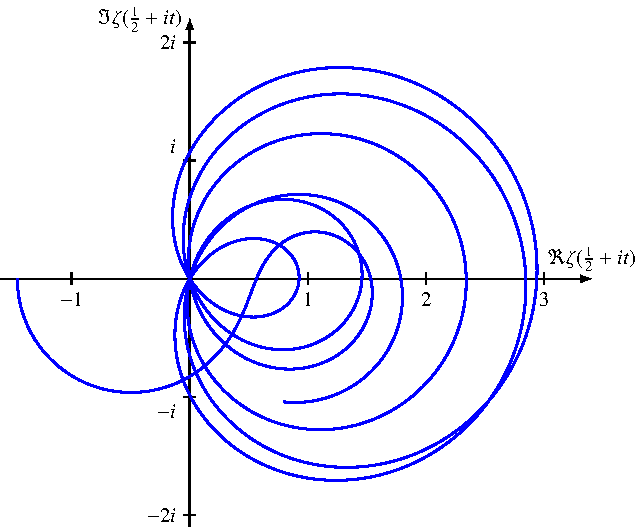
\includegraphics{papers/zeta/images/zetaplot.pdf}
    \caption{Die komplexen Werte der Zeta-Funktion für die kritische Gerade $\Re(s)=\frac{1}{2}$ im Bereich $\Im(s) = 0\dots40$.
    Klar sichtbar sind die immer wiederkehrenden Nullstellen, wie sie Gegenstand der Riemannschen Vermutung sind.}
    \label{zeta:fig:einzweitel}
\end{figure}


\printbibliography[heading=subbibliography]
\end{refsection}
